\documentclass{../llncs}
%%%%%%%%%%%%%%%%%%%%%%%%%%%%%%%%%%%%%%%%%%%%%%%%%%%%%%%%%%%
%% package sillabazione italiana e uso lettere accentate
% \usepackage[latin1]{inputenc}
\usepackage[utf8]{inputenc}
\usepackage[english]{babel}
\usepackage[T1]{fontenc}
%%%%%%%%%%%%%%%%%%%%%%%%%%%%%%%%%%%%%%%%%%%%%%%%%%%%%%%%%%%%%

% per gli elenchi
\usepackage{enumitem}

% https://en.wikibooks.org/wiki/LaTeX/Source_Code_Listings
%%%%%%%%%%%%%%%%%%%%%%%%%%%%
\usepackage{listings}

\usepackage{xcolor}
\definecolor{darkgreen}{HTML}{007700}

\lstset{
	basicstyle=\small\ttfamily,
	columns=fullflexible,
	keywordstyle=\color{violet}\bfseries,
	commentstyle=\color{darkgreen},
	breaklines=true,	 			% sets automatic line breaking
	captionpos=b,					% sets the caption-position to bottom
	stringstyle=\color{blue},     	% string literal style
	showstringspaces=false, 		% no special string spaces
	caption={\lstname},
	% title=\lstname,               % show the filename of files included with \lstinputlisting;
	numbers=left,
	numberstyle=\tiny,
	stepnumber=1,
	numbersep=5pt,
	frame=shadowbox
	% , float=*
}

\lstdefinestyle{style_qa}{
	language=C++,
	morekeywords={
		Plan,System,Event,Dispatch,Context,ip,host,port,httpserver,QActor,context,
		normal,switchTo,transition,whenMsg,finally,repeatPlan,stopAfter,resumeLastPlan,
		onMsg,addRule,replyToCaller,onEvent,removeRule,javaRun,whenTime,sendto,emit,else,not,
		selfMsg,forward,delay,whenEvent,printCurrentEvent,EventHandler,forwardEvent,Rules,demo
	}
}

\lstnewenvironment{qacode}[1][]{\lstset{style=style_qa, #1}}{}
% \begin{qacode}[caption={Programma Blink, "Hello World!"}]
% ...
% \end{qacode}
%%%%%%%%%%%%%%%%%%%%%%%%%%%%

\usepackage{url}
\usepackage{xspace}
\usepackage{color}
\makeatletter
%%%%%%%%%%%%%%%%%%%%%%%%%%%%%% User specified LaTeX commands.
\usepackage{../manifest}

\makeatother

% https://en.wikibooks.org/wiki/LaTeX/Hyperlinks
% LaTeXimpaziente: "Il pacchetto hyperref, che di regola va caricato per ultimo, crea i collegamenti ipertestualivall’interno del documento, rendendo cliccabili i riferimenti incrociati"
\usepackage{hyperref}

%%%%%%%
 \newif\ifpdf
 \ifx\pdfoutput\undefined
 \pdffalse % we are not running PDFLaTeX
 \else
 \pdfoutput=1 % we are running PDFLaTeX
 \pdftrue
 \fi
%%%%%%%
 \ifpdf
 \usepackage[pdftex]{graphicx}
 \else
 \usepackage{graphicx}
 \fi
%%%%%%%%%%%%%%%
 \ifpdf
 \DeclareGraphicsExtensions{.pdf, .jpg, .tif}
 \else
 \DeclareGraphicsExtensions{.eps, .jpg}
 \fi
%%%%%%%%%%%%%%%

\newcommand{\java}{\textsf{Java}}
\newcommand{\android}{\texttt{Android}}
\newcommand{\dsl}{\texttt{DSL}}
\newcommand{\jazz}{\texttt{Jazz}}
\newcommand{\rtc}{\texttt{RTC}}
\newcommand{\ide}{\texttt{Contact-ide}}
\newcommand{\xtext}{\texttt{XText}}
\newcommand{\xpand}{\texttt{Xpand}}
\newcommand{\xtend}{\texttt{Xtend}}
\newcommand{\pojo}{\texttt{POJO}}
\newcommand{\junit}{\texttt{JUnit}}

\newcommand{\action}[1]{\texttt{#1}\xspace}
% \newcommand{\codescript}[1]{{\scriptsize{\texttt{#1}}}\xspace}
\newcommand{\codescript}[1]{{\mbox{\small{\texttt{#1}}}}\xspace}
\newcommand{\code}[1]{{\color{blue}\small{\texttt{#1}}}}
\newcommand{\fname}[1]{{\small{\color{magenta}\texttt{#1}}}}
\newcommand{\node}{\textsf{NodeJs}}
\newcommand{\qa}{\textsf{\textit{QActor}}\xspace}

% Cross-referencing
\newcommand{\labelsec}[1]{\label{sec:#1}}
\newcommand{\xs}[1]{\sectionname~\ref{sec:#1}}
\newcommand{\xsp}[1]{\sectionname~\ref{sec:#1} \onpagename~\pageref{sec:#1}}
\newcommand{\labelssec}[1]{\label{ssec:#1}}
\newcommand{\xss}[1]{\subsectionname~\ref{ssec:#1}}
\newcommand{\xssp}[1]{\subsectionname~\ref{ssec:#1} \onpagename~\pageref{ssec:#1}}
\newcommand{\labelsssec}[1]{\label{sssec:#1}}
\newcommand{\xsss}[1]{\subsectionname~\ref{sssec:#1}}
\newcommand{\xsssp}[1]{\subsectionname~\ref{sssec:#1} \onpagename~\pageref{sssec:#1}}
\newcommand{\labelfig}[1]{\label{fig:#1}}
\newcommand{\xf}[1]{\figurename~\ref{fig:#1}}
\newcommand{\xfp}[1]{\figurename~\ref{fig:#1} \onpagename~\pageref{fig:#1}}
\newcommand{\labeltab}[1]{\label{tab:#1}}
\newcommand{\xt}[1]{\tablename~\ref{tab:#1}}
\newcommand{\xtp}[1]{\tablename~\ref{tab:#1} \onpagename~\pageref{tab:#1}}
% Category Names
\newcommand{\sectionname}{Section}
\newcommand{\subsectionname}{Subsection}
\newcommand{\sectionsname}{Sections}
\newcommand{\subsectionsname}{Subsections}
\newcommand{\secname}{\sectionname}
\newcommand{\ssecname}{\subsectionname}
\newcommand{\secsname}{\sectionsname}
\newcommand{\ssecsname}{\subsectionsname}
\newcommand{\onpagename}{on page}

\newcommand{\xauthA}{Filippo Frabetti}
\newcommand{\xauthB}{Nicola Semprini}
\newcommand{\xauthC}{Paolo Magnani}
\newcommand{\xfaculty}{II Faculty of Engineering}
\newcommand{\xunibo}{Alma Mater Studiorum -- University of Bologna}
\newcommand{\xaddrBO}{viale Risorgimento 2}
\newcommand{\xaddrCE}{via Venezia 52}
\newcommand{\xcityBO}{40136 Bologna, Italy}
\newcommand{\xcityCE}{47023 Cesena, Italy}

%
% Comments
%
% What’s wrong with \bf, \it, etc.? --> https://texfaq.org/FAQ-2letterfontcmd
% \newcommand{\todo}[1]{\bf{TODO:}\emph{#1}}
\newcommand{\todo}[1]{\textbf{TODO:} \emph{#1}}

\begin{document}

\title{Software Systems Engineering: Final task 2018}

\author{\xauthA, \xauthB, \xauthC}

\institute{%
  \xunibo\\\xaddrBO, \xcityBO\\
  \email{filippo.frabetti@studio.unibo.it}\\
  \email{nicola.semprini4@studio.unibo.it}\\
  \email{paolo.magnani5@studio.unibo.it}
}

\maketitle

% %%%%%%%%%%%%%%%%%%%%%%%% ABSTRACT + KEYWORDS - TODO... %%%%%%%%%%%%%%%%%%%%%%%%
\begin{abstract}
\footnotesize

This document is the explicit representation of the production process adopted.\\

\todo{abstract and keywords}

% (This part is optional)
%%This a Latex template to be used for the explicit representation of the production process adopted in the Software Systems Engineering course. 
% THIS DOCUMENT MUST FILL AT MOST TWO PAGES AND MUST BE PRINTED ON A SINGLE PAPER SHEET.

% The document can be compiled by using the \fname{kitISLatex.zip} given in \code{iss2018/it.unibo.issMaterial/issdocs/Lab}
  
\keywords{
% (This part is optional)
Software engineering, software development process, process representation, ...
}
\end{abstract}

% evita le righe eccessivamente lunghe aumentando la spaziatura tra le parole
% Il comando \fussy ripristina le impostazioni predefinite 
\sloppy

%===========================================================================
\section{Introduction}
\labelsec{intro}

L'ordine di presentazione delle sezioni in questo documento è solo parzialmente cronologico, in quanto spesso, durante il processo di sviluppo, è stato necessario rivedere le scelte fatte in precedenza alla luce di nuove considerazioni.
%===========================================================================

%===========================================================================
\section{Vision}
\labelsec{vision}

In fase di analisi e di progettazione scegliamo di procedere top-down, con zooming progressivo verso i dettagli.

Il processo di sviluppo adottato è di tipo \emph{Agile}, ovvero prediligendo ad ogni step la creazione di prototipi funzionanti da sottoporre al committente al fine di ottenere dei feedback.

In accordo con questa visione, anche i requisiti vengono affrontati in maniera incrementale.
%=========================================================================== 

%===========================================================================
\section{Requirements}
\labelsec{Requirements}

%With reference to a \texttt{mbot} physical robot working in a virtual environment, build an application that sends the data sensed by the virtual and the real sonars to the radar. More specifically:
%\begin{itemize}
%\item[-]the data of the \emph{virtual sonar} \texttt{sonar1} must be displayed on the direction of angle=\fname{30};
%\item[-]the data of the \emph{virtual sonar} \texttt{sonar2} must be displayed on the direction of angle=\fname{120};
%\item[-]the data of the \emph{virtual sonar} on the virtual robot must be displayed on the direction of angle=\fname{90} at the fixed distance of \fname{40};
%\item[-]the data of the \emph{real sonar} on the physical robot must be displayed on the direction of angle=\fname{0};
%\end{itemize}

% 13 - A new problem
%\begin{enumerate}
%\item The physical robot must expose in a visible way a \code{Led} and:
%\begin{itemize}
%\item[-] the Led must be \code{on} when the robot is engaged by an user (human or machine);
%\item[-] the Led must be \code{off} when the robot is available for booking.
%\end{itemize}
%\item the robot system does not expose any public available usage interface;
%\item in order to use the robot, an user must first of all send 'to the system' a \code{booking request}. The system
%must return an answer including an \code{access token} if the robot is available. If the answer is negative, (robot
%already engaged) and the request includes a '\texttt{notify-me flag}', the system must notify the user when to robot
%becomes again available;
%\item the user that receives the \code{access token} must send within a given \code{acquisition-deadline} (e.g. \code{30 sec}) the request for a \emph{robot-driving command interface}, by appending to the request the \code{access token}. If the
%\emph{acquisition-deadline} expires, the robot returns in its 'available state';
%\item the user can use the \emph{robot-driving command interface} at most for a prefixed \code{usage-duration} time;
%\item the user can explicitly release the robot resource by sending a \code{booking release} message;
%\item if many users attempt to book the robot resource 'at the same time', the system could operate in two different
%ways:
%\begin{itemize}
%\item[(a)] by selecting the first \emph{emitted} request;
%\item[(b)] by selecting the first \emph{received} request
%\end{itemize}
%\end{enumerate}

% FINAL TASK 2018
In a home of a given city (e.g. Bologna), a \texttt{ddr} robot is used to clean the floor of a room (\code{R-FloorClean}).

The floor in the room is a flat floor of solid material and is equipped with two \emph{sonars}, named \code{sonar1} and \code{sonar2} as shown in the picture
\footnote{\textit{iss2018$\backslash$it.unibo.issMaterial$\backslash$issdocs$\backslash$Material$\backslash$nodeLab2018.pdf}: \textbf{8 Final task 2018}}
(\code{sonar1} is that at the top). The initial position (\code{start-point}) of the robot is detected by \code{sonar1}, while the final position (\code{end-point}) is detected by \code{sonar2}.\\

\noindent The robot works under the following conditions:
\begin{enumerate}
\item \code{R-Start}: an \code{authorized user} has sent a \texttt{START} command by using a human \texttt{GUI} interface (\code{console}) running on a conventional PC or on a smart device (\texttt{Android}).
\item \code{R-TempOk}: the value temperature of the city is not higher than a prefixed value (e.g. \texttt{25} degrees Celsius).
\item \code{R-TimeOk}: the current clock time is within a given interval (e.g. between \texttt{7} a.m and \texttt{10} a.m).
\end{enumerate}

\noindent While the robot is working:
\begin{itemize}[label={--}]
\item it must blink a \texttt{Led} put on it, if the robot is a \fname{real} robot (\code{R-BlinkLed}).
\item it must blink a \texttt{Led Hue Lamp} available in the house, if the robot is a \fname{virtual} robot (\code{R-BlinkHue}).
\item it must avoid fixed obstacles (e.g. furniture) present in the room (\code{R-AvoidFix}) and/or mobile obstacles like
balls, cats, etc. (\code{R-AvoidMobile}).
\end{itemize}

Moreover, the robot must stop its activity when one of the following conditions apply:
\begin{enumerate}
\item \code{R-Stop}: an \code{authorized user} has sent a \texttt{STOP} command by using the \code{console}.
\item \code{R-TempKo}: the value temperature of the city becomes higher than the prefixed value.
\item \code{R-TimeKo}: the current clock time is beyond the given interval.
\item \code{R-Obstacle}: the robot has found an obstacle that it is unable to avoid.
\item \code{R-End}: the robot has finished its work.
\end{enumerate}

%During its work, the robot can optionally:
%\begin{itemize}[label={--}]
%\item \code{R-Map}: build a map of the room floor with the position of the fixed obstacles. Once built, this map can be
%used to define a plan for an (optimal) path form the \code{start-point} to the \code{end-point}.
%\end{itemize}
%
%Other requirements:
%\begin{enumerate}
%\item The work can be done by a team composed of \code{NT} people, with \code{1<=NT<=4}.
%\item If \code{NT>1}, the team must explicitly indicate the work done by each component.
%\item If \code{NT==4}, the requirement \code{R-Map} is mandatory.
%\end{enumerate}
%===========================================================================

%===========================================================================
\section{Requirement analysis}
\labelsec{ReqAnalysis}
Dai requisiti emerge il fatto che il sistema sia distribuito e composto da due nodi di esecuzione: uno per il robot ed uno che ospita la logica di controllo e fornisce la console, usabile da remoto, per pilotare il robot (\code{R-Start} e \code{R-Stop}).\\

\noindent Si delineano nello specifico 5 entità:
\begin{enumerate}
\item il robot, che può essere sia fisico sia virtuale (\texttt{RealRobot} e \texttt{VirtualRobot}), e l'ambiente in cui si muove (fisico/virtuale)
\item gli attuatori: il \texttt{Led} per il robot reale e l'\texttt{HueLamp} per quello virtuale
\item i sensori: un indicatore di temperatura remoto (\texttt{RemoteThermometer}) e un orologio (\texttt{ClockAgent})
\item un utilizzatore umano (\texttt{HumanOperator}) a cui è collegata la console grafica
\item un componente che andrà ad incapsulare l'\texttt{Application logic}
\end{enumerate}

\noindent L'ambiente in cui si trova il robot è inoltre costituito da:
\begin{itemize}[label={--}]
\item 2 sensori \code{sonar1} e \code{sonar2} % (ambiente virtuale) %% sono virtuali solo perchè non li abbiamo fisici, giusto?
\item ostacoli fissi (pareti) e mobili
\end{itemize}

L'architettura del sistema può essere quindi descritta in maniera informale dalla \xf{informalRA}.
\begin{figure}[!htb]
\centering
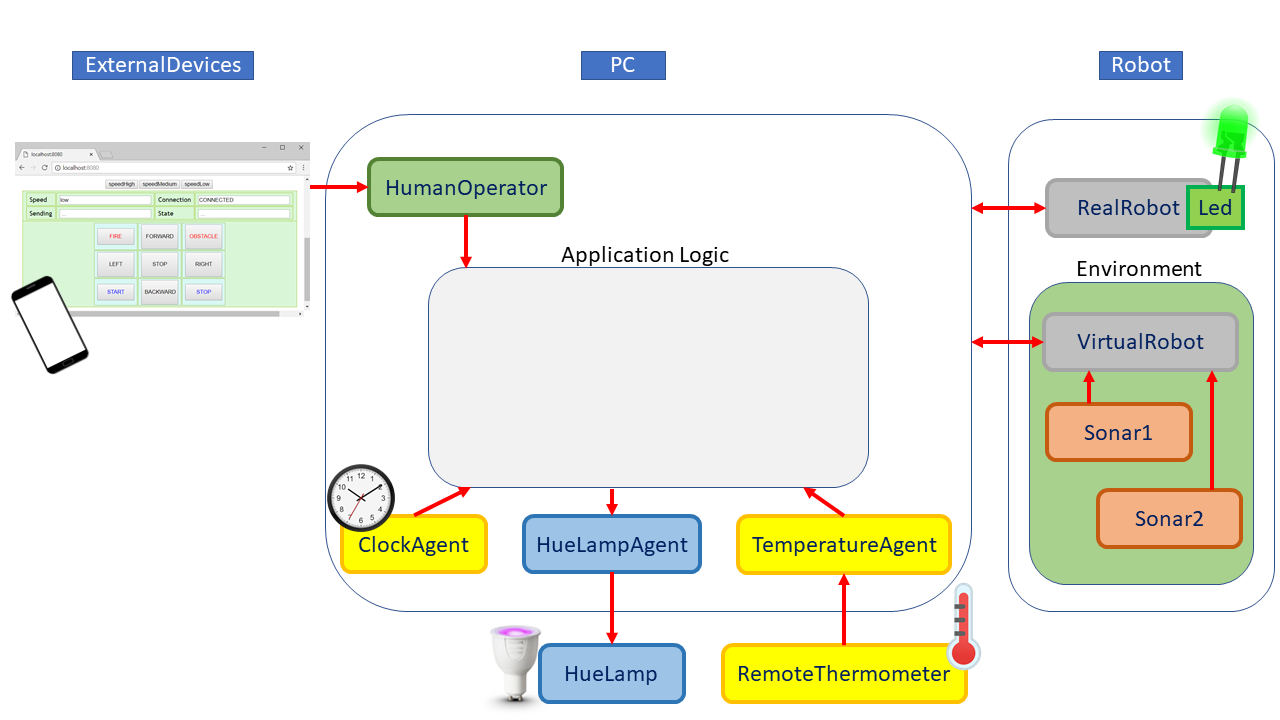
\includegraphics[scale=0.4]{img/informalArchitecture1.png}
\caption{Architettura informale ottenuta dall'analisi dei requisiti}\labelfig{informalRA}
\end{figure}

\vspace{8px}

Passiamo ora ad analizzare formalmente i singoli componenti presenti all'interno dei due contesti, a partire da quello che rappresenta l'applicazione principale.

\subsection{Actuators}
\labelssec{actuatorsRA}
Il \texttt{Led}, essendo un componente estremamente semplice e trovandosi sul robot fisico, può essere visto come un'entità passiva senza un proprio flusso di controllo. Pertanto, il modello del \texttt{Led} -- un oggetto Java -- può essere formalmente definito dalla seguente interfaccia:

\begin{center}
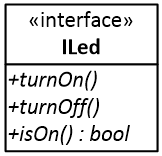
\includegraphics[scale=0.4]{img/iled.png}
\end{center}

L'interazione con il \texttt{Led} può quindi avvenire tramite \textit{procedure call} ad opera del robot fisico su cui si trova.\\

L'\texttt{Hue Lamp} è invece un'entità attiva che ci viene fornita dal committente insieme ad un componente software per poter interagire con essa attraverso un'interfaccia \textit{RESTful}
\footnote{\url{https://www.developers.meethue.com/philips-hue-api}}.

Possiamo quindi definire il modello di un attore in grado di interagire con l'\texttt{Hue Lamp} remota: per farlo usiamo il linguaggio custom della nostra Software House \qa, poiché ci permette di modellare sistemi distribuiti eterogenei.\\

\lstinputlisting[style=style_qa, firstline=18, lastline=37, firstnumber=18]{../it.unibo.finalTask2018/src/requirementsAnalysis.qa}

Si noti come la scelta di utilizzare l'evento \codescript{lightCmd} consenta di controllare più dispositivi senza che questi siano noti a priori dalla sorgente che emette tali eventi in base alla logica applicativa.

Inoltre, poiché i comandi utilizzati nel payload dell'evento non si limitano al solo \textit{lampeggiamento}, il modello è generale e facilmente riutilizzabile. Ad esempio un cambiamento dei requisiti potrebbe stabilire che il led debba restare acceso durante il movimento del robot.

\subsection{Sensors}

\subsubsection{TemperatureAgent}
Poiché abbiamo a che fare con un servizio remoto che fornisce i dati sulla temperatura, modelliamo un attore che funga da \emph{adapter} e permetta la comunicazione tra questi e il sistema.\\

In generale, l'applicazione può interagire con l'adapter mediante tre possibili approcci del tipo produttore/consumatore:
\begin{itemize}
\item \textbf{polling:} chi necessita dell'informazione si fa carico di fare richiesta periodicamente al consumatore;
\item \textbf{pattern observer:} l'observer si registra presso l'observable e viene notificato al cambiamento di stato di quest'ultimo;
\item \textbf{publish/subscribe:} è il produttore stesso a pubblicare all'esterno le informazioni quando queste sono disponibili, ad uso degli eventuali consumatori.
\end{itemize}
Scegliamo di adottare la terza strategia, poiché meno costosa in termini di dati scambiati e poiché garantisce un minor accoppiamento tra le entità coinvolte.

Nell'ambiente distribuito in cui operano i QActor, la pubblicazione (\textit{publish}) di informazioni avviene tramite l'emissione di \textbf{eventi} che per essere rilevati necessitano che il consumatore si sia preventivamente messo in ascolto (operazione logicamente equivalente alla \textit{subscribe}).\\

\lstinputlisting[style=style_qa, firstline=41, lastline=55, firstnumber=41]{../it.unibo.finalTask2018/src/requirementsAnalysis.qa}

Come per \codescript{lightCmd}, anche in questo caso l'evento \codescript{temperature}% : temperature(T)}
emesso dall'adapter del sensore può essere percepito da chiunque sia in ascolto, senza dover specificare a priori i possibili componenti interessati.\\

Si noti infine come l'interazione tra \codescript{TemperatureAgent} e il servizio che fornisce la temperatura sia a polling.

\subsubsection{ClockAgent}
% Poiché nei requisiti non viene specificata la natura del \texttt{Clock},
Per quanto riguarda il \texttt{Clock}, scegliamo di modellarlo come un attore a se stante, separato dalla logica applicativa specifica del problema, così che sia facilmente modificabile e riutilizzabile.%; inoltre, in questo modo in futuro potrebbe essere tranquillamente sostituito con un meccanismo di sincronizzazione distribuito (es. orologio logico di Lamport\footnote{\url{https://en.wikipedia.org/wiki/Leslie_Lamport}}).

Il modello di tale attore è pressoché analogo a quello visto per \texttt{TemperatureAgent}.\\

\lstinputlisting[style=style_qa, firstline=59, lastline=74, firstnumber=59]{../it.unibo.finalTask2018/src/requirementsAnalysis.qa}

\subsection{HumanOperator}
\labelssec{humanOpRA}
Lo \texttt{HumanOperator} può essere modellato come un emettitore di comandi per il robot. Per disaccoppiare le comunicazioni tra sorgente e destinatario dei comandi, l'operator si rivolge ad una terza entità che rappresenta la logica applicativa, così da non essere vincolato a conoscere l'identità di ogni possibile robot pilotabile.

Si noti come tale disaccoppiamento funziona anche al contrario: gli eventuali robot possono essere pilotati il maniera uniforme da molteplici sorgenti di comandi, tutte facenti riferimento alla stessa application logic. Nel nostro caso ciò si verifica per l'utilizzatore umano (\texttt{HumanOperator}) e per l'agente software che muove il robot in autonomia per la pulizia della stanza (\texttt{SoftwareAgent}, vedi \xss{swagPA}).\\

\lstinputlisting[style=style_qa, firstline=78, lastline=92, firstnumber=78]{../it.unibo.finalTask2018/src/requirementsAnalysis.qa}

In questa prima fase di modellazione, lo \texttt{HumanOperator} va a generare programmaticamente i comandi per il robot. In un secondo momento questi saranno invece originati da un effettivo utente umano che utilizza una console grafica (\xss{humanOpPA}).

\subsection{Application logic}
Per poter attuare la logica applicativa stabilita dai requisiti, l'applicazione deve ricevere i dati della temperatura, del tempo e dei vari sonar, emessi sotto forma di eventi; oltre a questi, deve mettersi in attesa dei comandi di movimento inviati dallo \texttt{HumanOperator}, così da poterli inoltrare a tutti i robot disponibili (reali e virtuali): a tal fine è stato introdotto l'evento \codescript{robotCmd : moveRobot(CMD)}.

Sempre in accordo con i requisiti, l'applicazione deve gestire ed emettere, quando opportuno, gli eventi contenenti i comandi che regolano il \texttt{Led}, presente sul robot fisico, e la \texttt{Hue Lamp} remota, gestita da quello virtuale.\\

\lstinputlisting[style=style_qa, firstline=96, lastline=119, firstnumber=96]{../it.unibo.finalTask2018/src/requirementsAnalysis.qa}

\subsection{Robot}
\labelssec{robotRA}
Ci viene fornito un modello del robot espresso nel linguaggio \qa
\footnote{iss2018Lab/it.unibo.mbot.divide/src/realRobotExecutor.qa e virtualRobotExecutor.qa}: questi è in grado di ricevere messaggi \codescript{moveRobot : moveRobot(CMD)} e di interpretarli come comandi di movimento (forward, backward, left, right, stop).

Il robot è anche dotato di un sonar frontale che gli permette di rilevare la presenza di ostacoli (\code{R-AvoidFix} e \code{R-AvoidMobile}), rivestendo il duplice ruolo di attuatore e di sensore, in quanto emette informazioni relative alla distanza dagli ostacoli che incontra sotto forma di eventi \codescript{frontSonar : sonar(DISTANCE)}.

Il robot è quindi un'entità attiva il cui scopo è interpretare i messaggi ricevuti in un certo formato ed emettere eventi relativi al sonar frontale.\\

Poiché l'attore che incarna la logica applicativa emette comandi sotto forma di eventi \codescript{robotCmd}, è necessario introdurre un ulteriore componente che effettui il mapping di questi nei rispettivi messaggi \codescript{moveRobot} gestiti dal robot. In questo caso, dal momento che vogliamo evitare che i comandi per pilotare il robot vadano persi, facciamo ricorso per tale scopo ad un componente \emph{event-driven} (\texttt{EventHandler}).\\

\lstinputlisting[style=style_qa, lastline=42]{../it.unibo.finalTask2018/src/ddr.qa}

L'implementazione delle varie mosse viene delegata ad un'opportuna classe Java, così che questa possa essere modificata senza alterare il modello del robot. Questa soluzione permette inoltre di riutilizzare lo stesso modello per entrambe le tipologie di robot, reale e virtuale.\\

Nella stanza sono presenti due sonar in grado di rilevare la presenza di un robot che passi in corrispondenza di uno dei due, emettendo in tal caso un evento \codescript{sonarSensor : sonar(NAME,DISTANCE)}, dove \codescript{NAME} è \code{sonar1} o \code{sonar2}.

L'emissione di tali eventi dipende dalla specifica implementazione dell'\textit{environment}, pertanto anch'essa viene delegata ad una classe Java:\\

\lstinputlisting[language=Java, firstline=9, lastline=21, firstnumber=9]{../it.unibo.finalTask2018/src/it/unibo/finalTask2018/ra/robotAdapter.java}

\subsection{System formal definition}
\labelssec{formalRA}
L'immagine della \xf{informalRA} può essere quindi formalmente definita dal sistema {\qa} risultante dall'integrazione tra \codescript{ddr.qa} e \codescript{requirementsAnalysis.qa}, rappresentata da un ulteriore componente il cui compito è mettere in contatto i contesti degli altri due.\\

\lstinputlisting[style=style_qa, lastline=14]{../it.unibo.finalTask2018/src/raintegrator.qa}

In alternativa, è possibile decommentare in \codescript{ddr.qa} la riga contenente la conoscenza del contesto dell'applicazione principale, aggiungendo quindi il vincolo che al momento dell'esecuzione del robot questa sia già attiva.

Questa seconda opzione è meno conveniente dal punto di vista del testing automatizzato dei singoli componenti, discusso nella \xsss{reqAnalTesting}.\\

\vspace{8px}

Poiché abbiamo utilizzato un \emph{modello eseguibile}, questo ci fornisce anche un primo \textbf{prototipo} funzionante della nostra applicazione.

\subsection{Cleaning the room}
Ora che l'architettura del sistema è formalmente definita, passiamo ad analizzare il requisito fondamentale: \code{R-FloorClean}.\\

Pulire la stanza significa trovare un percorso da un punto di partenza (\code{start-point}) ad un punto di arrivo (\code{end-point}) predefiniti che copra l'intera superficie disponibile. Ciò può essere fatto in svariati modi, tuttavia si considera desiderabile impiegare il minor tempo possibile e quindi limitare il passaggio ripetuto per le stesse posizioni già pulite in precedenza.

Consideriamo inizialmente una stanza rettangolare e priva di ostacoli. In questo caso esistono più percorsi che consentono di non passare mai due volte per lo stesso punto: ad esempio procedendo a spirale lungo le pareti e proseguendo verso il centro della stanza, oppure a ``zig-zag'' parallelamente ad una parete, avvicinandosi via via a quella opposta.

La differenza sostanziale tra le due risiede nella posizione finale: nella prima questa si trova al centro della stanza, mentre nella seconda lungo la parete opposta a quella di partenza. Da notare come nella seconda alternativa, data la specifica della stanza e la collocazione dei due sonar fissi, il punto di arrivo coincida con \code{sonar2}.\\

\begin{center}
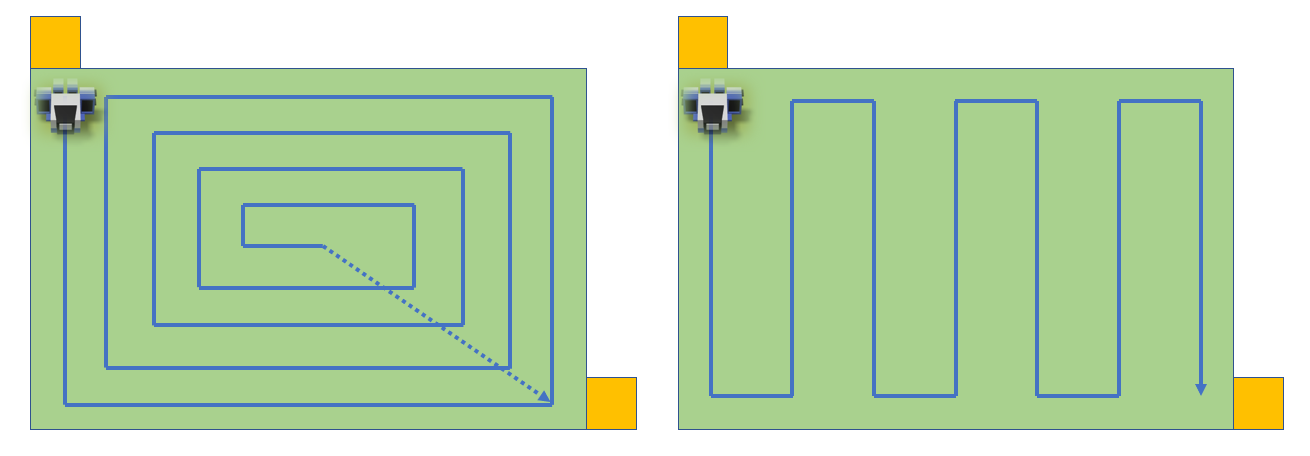
\includegraphics[scale=0.4]{img/roomMap.png}
\end{center}

L'assunzione relativa alla forma rettangolare della stanza non è assolutamente restrittiva, mentre la presenza di eventuali ostacoli riguarda i requisiti trattati di seguito.

\subsubsection{R-End}
Il robot deve fermarsi quando ha terminato la pulizia dell'intera stanza. Ciò significa, in altre parole, aver percorso almeno una volta tutti i punti della superficie. Ci chiediamo come sia possibile verificare questo requisito.

Se conoscessimo le dimensioni della stanza, basterebbe tenere traccia del percorso seguito per controllare la superficie coperta dal robot. Un modo per fare ciò potrebbe essere rappresentare la stanza come una scacchiera composta da un reticolo di celle quadrate che il robot può percorrere con una mossa elementare (un ``passo''). La dimensione delle celle deve essere sufficientemente piccola per essere vicina a un numero divisibile per le due dimensioni della stanza, così da limitare la presenza di ``mezzi-passi'', ma anche abbastanza grande da essere misurabile dal robot.

L'unico modo che il robot ha a disposizione per misurare le distanze è tramite il tempo, ovvero, assumendo di muoversi a velocità costante (trascurando l'accelerazione dovuta alla partenza e allo stop), lo spazio percorso è dato dalla legge:
\[s = v t \]

Il robot quindi, muovendosi all'interno della griglia, può tenere traccia di tutti i passi fatti così da poter verificare in seguito di essere passato almeno una volta su ogni casella. Questo comporta però di conoscere prima la dimensione della stanza.\\

Un'alternativa è assumere che, adottando il movimento a ``zig-zag'', quando il robot viene rilevato molto vicino a \code{sonar2} questi abbia pulito l'intera stanza. Ciò è sicuramente vero nel caso di una semplice stanza rettangolare e priva di ostacoli, la cui lunghezza è multiplo pari del ``passo laterale'' compiuto dal robot al termine di ogni rettilineo.

\subsubsection{R-Start and R-Stop}
% cosa vuol dire utente autorizzato

% console utilizzabile da qualsiasi dispositivo -> web server
%===========================================================================

%===========================================================================
\section{Problem analysis}
\labelsec{ProblemAnalysis}
Il problema definito dai requisiti si colloca nell'ambito dell'IoT, dove è diffuso l'utilizzo della cosiddetta \emph{architettura esagonale} come design pattern per gestire il rapporto tra input, elaborazione ed output nei sistemi distribuiti. In tale pattern, un ruolo centrale viene rivestito dalla \emph{business logic} e dal modello delle risorse (\emph{resource model}), mentre gli altri componenti del sistema vengono visti tramite degli adapter verso le varie tecnologie ed implementazioni.

Il modello delle risorse è quindi un disaccoppiatore del mondo fisico da quello della logica applicativa, che deve essere indipendente dalla tecnologia. Nello specifico:
\begin{enumerate}
\item un cambiamento dello stato del sensore fisico causa un cambiamento dello stato del modello del sensore stesso
\item al cambiamento del modello, l'informazione viene notificata al controller (è un observer del modello)
\item il controller modifica quindi il modello dell'attuatore in base alla logica applicativa
\item l'aggiornamento del modello dell'attuatore comporta infine un aggiornamento dell'attuatore fisico
\end{enumerate}

Come analisti riteniamo vantaggioso introdurre un modello delle risorse così da non vincolare la logica applicativa a dettagli tecnologico-implementativi, sebbene ciò comporti un piccolo sforzo aggiuntivo iniziale. Tale overhead è però un investimento a fronte dello sviluppo futuro di applicazioni simili, inoltre, se il modello fosse standardizzato, sarebbe garantita l'interoperabilità tra sistemi diversi.

\subsection{Resource Model}
Per la definizione del modello delle risorse usiamo un linguaggio dichiarativo che consenta di esprimere sia lo stato di ciascun componente, sia le operazioni primitive su di esso. A tal fine, introduciamo il seguente modello scritto in Prolog:\\

\lstinputlisting[language=Prolog, keywordstyle=\color{black}, lastline=36]{../it.unibo.finalTask2018/resourceModel.pl}

\subsection{Logical architecture}
In seguito all'introduzione del modello delle risorse possiamo definire l'architettura logica del sistema in modo informale tramite la \xf{informalLA}.

\begin{figure}[!htb]
\centering
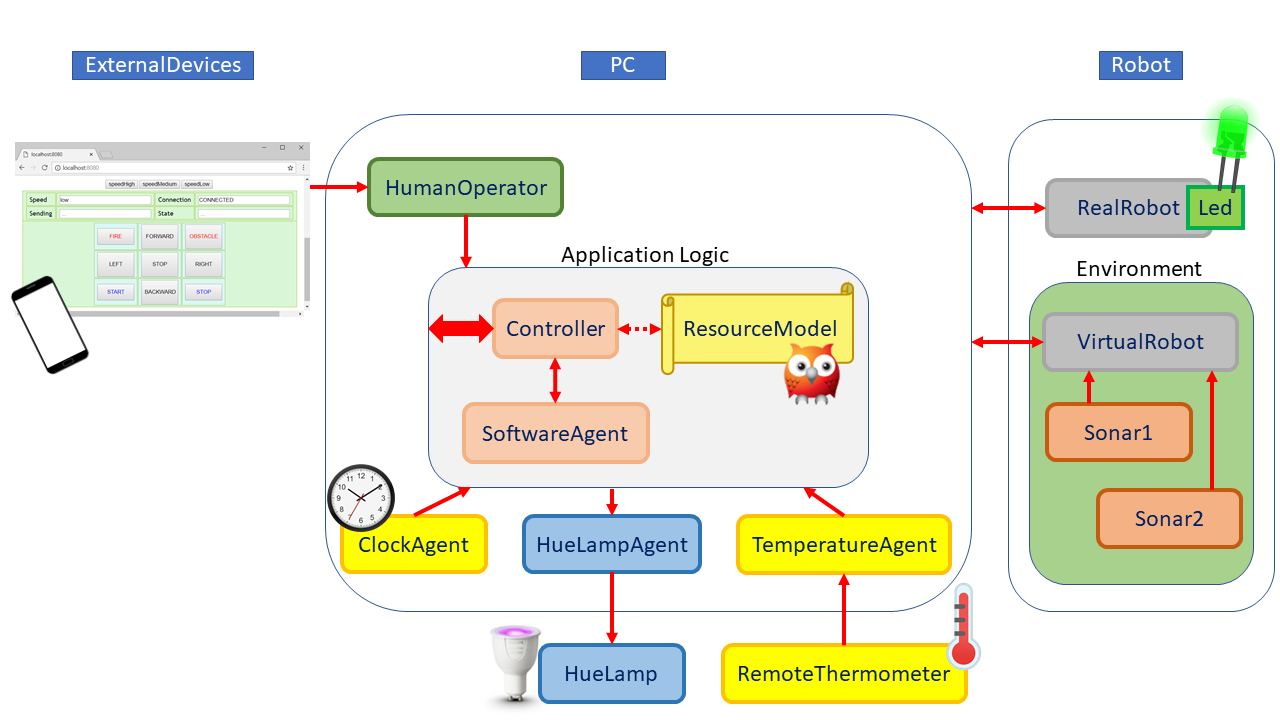
\includegraphics[scale=0.4]{img/informalArchitecture2.png}
\caption{Architettura logica informale}\labelfig{informalLA}
\end{figure}

Rispetto all'architettura risultante dall'analisi dei requisiti sono stati inoltre aggiunti i componenti \texttt{Controller} e \texttt{SoftwareAgent}.

\subsection{Controller}
Il ruolo del \texttt{Controller} è quello di gestire il modello delle risorse in base ai dati ricevuti dai sensori e alla logica applicativa, in accordo con il pattern MVC: resource model, sensori/attuatori e controller.

Modelliamo quindi il \texttt{Controller} come un attore in grado di ricevere in input informazioni dagli altri componenti del sistema ed emettere in output comandi sotto forma di eventi \codescript{ctrlEvent : ctrlEvent(CATEG,NAME,CMD)}.\\

\lstinputlisting[style=style_qa, lastline=19]{../it.unibo.finalTask2018/src/problemAnalysis.qa}

Tramite un \emph{EventHandler}, ogni evento emesso dai sensori viene mappato in un evento \codescript{inputCtrlEvent : inputEvent(CATEG,NAME,VALUE)} ad uso interno del \texttt{Controller}, così che eventi provenienti da sensori fisici diversi possano essere trattati allo stesso modo e non venire mai persi, % (a meno che le operazioni compiute dal \texttt{Controller} non richiedano troppo tempo),
essendo l'\emph{EventHandler} un componente event-driven.

Per discriminare la natura degli eventi ricevuti, il \texttt{Controller} può usare i campi \codescript{CATEG} e \codescript{NAME} presenti nel payload.\\

Come già anticipato, ad ogni modifica del Resource Model relativa allo stato di un attuatore, il \texttt{Controller} emette a sua volta degli eventi \codescript{ctrlEvent} per notificare il cambiamento ai vari attuatori fisici.\\

\lstinputlisting[style=style_qa, firstline=29, lastline=122, firstnumber=29]{../it.unibo.finalTask2018/src/problemAnalysis.qa}

Attualmente sono soddisfatti i requisiti \code{R-TempOk} e \code{R-TimeOk}, in quanto il \texttt{Controller} blocca ogni modifica allo stato del robot al di fuori di un certo intervallo temporale o in presenza di temperature troppo elevate. Il robot viene inoltre fermato non appena queste condizioni non sono più verificate (\code{R-TempKo} e \code{R-TimeKo}).

Oltre a questo, sono anche soddisfatti i requisiti relativi al lampeggiamento del \texttt{Led} e della \texttt{HueLamp} (\code{R-BlinkLed} e \code{R-BlinkHue}), dal momento che alla modifica del modello del robot segue l'emissione di un opportuno evento \codescript{ctrlEvent} ad uso degli attuatori della categoria ``led'', mappato poi da un apposito \emph{EventHandler} nel rispettivo evento \codescript{lightCmd}.\\

\lstinputlisting[style=style_qa, firstline=20, lastline=22, firstnumber=20]{../it.unibo.finalTask2018/src/problemAnalysis.qa}

\subsection{Software Agent}
\labelssec{swagPA}
\texttt{SoftwareAgent} realizza la logica applicativa in collaborazione con il \texttt{Controller}, occupandosi di manovrare il robot secondo il vincolo \code{R-FloorClean}. Decidiamo quindi di modellarlo come un attore nel suo stesso contesto.

L'agent si mette in ascolto degli eventi provenienti dai vari sonar e invia opportuni messaggi \codescript{cmd} al controller, gli stessi utilizzati da \texttt{HumanOperator} per muovere il robot.\\

In una fase preliminare, per motivi di testing, \texttt{SoftwareAgent} fa semplicemente ruotare il robot quando esso viene rilevato dai sonar a distanza ravvicinata.\\

\lstinputlisting[style=style_qa, firstline=126, lastline=175, firstnumber=126]{../it.unibo.finalTask2018/src/problemAnalysis.qa}

\subsection{Changes to HumanOperator}
\labelssec{humanOpPA}
Il sistema deve inoltre fornire un'interfaccia grafica per permettere l'interazione con l'utente da qualsiasi dispositivo (\code{R-Start}). Ciò può essere realizzato in prima battuta tramite l'inserimento del flag \codescript{-httpserver} nel contesto dell'applicazione, sfruttando il server HTTP fornito dall'infrastruttura \qa, con l'idea di poterlo sostituire in futuro con un server più sofisticato (ad esempio per realizzare l'autenticazione degli utenti richiesta nei requisiti \code{R-Start} e \code{R-Stop}).\\

\lstinputlisting[style=style_qa, firstline=14, lastline=14, firstnumber=14]{../it.unibo.finalTask2018/src/problemAnalysis.qa}

La GUI web ottenuta tramite il flag \codescript{-httpserver} è dotata di bottoni che, quando vengono premuti, scatenano eventi \codescript{usercmd : usercmd(robotgui(X))}. Lo \texttt{HumanOperator} deve quindi catturare questi eventi e inoltrarli sotto forma di messaggi \codescript{cmd : cmd(X)} al \texttt{Controller}.

Lo \texttt{HumanOperator} è ancora un emettitore di comandi per il robot come visto nella sezione precedente, tuttavia ora è in grado di generarli in base ai pulsanti premuti dall'utilizzatore umano sulla console.\\

\lstinputlisting[style=style_qa, firstline=179, lastline=194, firstnumber=179]{../it.unibo.finalTask2018/src/problemAnalysis.qa}

\subsection{Changes to Robot}
Il robot si mette in attesa di messaggi \codescript{moveRobot} e li interpreta come comandi di movimento, tuttavia i cambiamenti nel modello del robot vengono notificati all'esterno dal controller sotto forma di eventi \codescript{ctrlEvent}.

Similmente a quanto fatto nella \xss{robotRA}, per effettuare la conversione da \codescript{ctrlEvent} a messaggi abbiamo utilizzato un \emph{EventHandler}, così da accodare gli eventi senza il rischio di perderne qualcuno.\\ % (il robot è quindi, nel suo complesso, un componente \emph{event-driven}).\\

\lstinputlisting[style=style_qa, lastline=18]{../it.unibo.finalTask2018/src/virtualRobotNode.qa}

Poiché gli \emph{EventHandler} possono solo convertire eventi in messaggi con lo stesso payload, introduciamo un ulteriore evento \codescript{local\_robotCmd : moveRobot(CMD)} ad uso interno dei due \emph{EventHandler} che effettuano il mapping.
%l'attore \texttt{nodebroker}, il cui compito è quello di convertire i messaggi \codescript{ctrlMsg : ctrlEvent(CATEG, NAME, CMD)} inviati dall'\emph{EventHandler} in messaggi \codescript{moveRobot : moveRobot(CMD)} per il robot virtuale.\\

%\lstinputlisting[style=style_qa, firstline=52, lastline=57, firstnumber=52]{../it.unibo.finalTask2018/src/virtualRobotNode.qa}

\subsubsection{Virtual Robot with Node.js}
\labelssec{virtualRobotPA}
Concettualmente, il modello del robot virtuale è esattamente lo stesso della \xss{robotRA}. L'unica differenza risiede nella diversa implementazione dei metodi Java chiamati con il comando \codescript{javaRun}: in questo caso la classe Java dovrà connettersi con il server Node (dopo averlo avviato) e tradurre i comandi di movimento ricevuti in opportuni messaggi da inviare sulla connessione TCP. Sempre dalla stessa connessione riceverà, in un certo formato, i dati relativi ai vari sonar.

Si rimanda questo argomento più nel dettaglio nella \xss{robotNodeImpl}.

\subsubsection{Real Robot mock}
Per quanto riguarda il robot fisico, questi viene al momento simulato tramite un oggetto Java che si limita a stampare a video i comandi ricevuti.

Un attore a parte si occupa invece di gestire lo stato del led, anch'esso rappresentato da un oggetto mock.\\

\lstinputlisting[style=style_qa, firstline=44, lastline=55, firstnumber=44]{../it.unibo.finalTask2018/src/realRobotMock.qa}

\vspace{8px}

Da notare come entrambi i robot, reagendo agli stessi eventi \codescript{ctrlEvent} generati al cambiamento del modello del robot, possono eseguire in contemporanea le medesime mosse.
%===========================================================================

%===========================================================================
\section{Project}
\labelsec{Project}
Al momento, l'applicazione è in grado di soddisfare i seguenti requisiti:
\begin{itemize}
\item \code{R-TempOk}, \code{R-TimeOk}, \code{R-TempKo} e \code{R-TimeKo}, ad opera di opportune regole Prolog presenti nella base di conoscenza del \texttt{Controller}
\item \code{R-BlinkLed} e \code{R-BlinkHue}
\footnote{Resta da sviluppare l'implementazione della classe Java \emph{technology-dependent} che dovrà interagire in modo RESTful con la \texttt{Hue Lamp} remota}, mediante l'emissione da parte del controller di eventi \codescript{ctrlEvent : ctrlEvent(led,l1,CMD)} a seguito della modifica del modello del led \codescript{l1} in base allo stato di movimento del robot. L'Hue Lamp agent e il robot fisico sono sensibili a questo evento.
\end{itemize}

Rimangono da affrontare i restanti requisiti relativi al movimento autonomo del robot (pilotato da \texttt{SoftwareAgent}):
\begin{enumerate}
\item \code{R-Start} e \code{R-Stop}: la pulizia della stanza inizia e termina preventivamente a seguito di comandi \texttt{start/stop} inviati da un \emph{utente autorizzato}
\item \code{R-FloorClean} e \code{R-End}: il robot deve pulire l'intera superficie della stanza (da \code{sonar1} a \code{sonar2}), fermandosi al termine del lavoro
\item \code{R-AvoidMobile}, \code{R-AvoidFix} e \code{R-Obstacle}: il robot deve essere in grado di rilevare ed evitare gli ostacoli sia fissi sia mobili, eventualmente fermandosi nel caso ciò non sia possibile
\end{enumerate}

\subsection{Starting and stopping the agent}
Al momento è disponibile una \emph{web GUI} fornita dall'infrastruttura \qa grazie alla presenza del flag \codescript{-httpserver} presente nel contesto dell'applicazione. Questa è in grado di emettere eventi \codescript{usercmd : usercmd(CMD)} alla pressione dei pulsanti di movimento da parte dell'utilizzatore umano.

Oltre ai bottoni che corrispondono ai movimenti elementari del robot, ve ne sono altri due che possono essere utilizzati per l'avvio e la terminazione della pulizia della stanza ad opera di \texttt{SoftwareAgent}, con l'idea di gestire in seguito la problematica relativa all'autenticazione degli utenti.

Attualmente, la GUI di default emette eventi \codescript{cmd : cmd(C)} alla pressione di questi pulsanti. Abbiamo però deciso di sostituirli con eventi \codescript{alarm : usercmd(C)} così che, avendo lo stesso payload degli altri, la loro gestione risulti semplificata.\\

Poiché non vogliamo che nessun comando vada perso, introduciamo un componente event-driven (\emph{EventHandler}) che effettui un mapping degli eventi \codescript{alarm} in messaggi \codescript{externalcmd} diretti all'agent e aventi lo stesso payload dei precedenti.

\subsubsection{R-Start e R-Stop}
Alla pressione del pulsante di start, il robot deve trovarsi vicino a \code{sonar1} per poter partire con la pulizia, in caso contrario il comando viene ignorato. Se invece viene ricevuto un messaggio di stop (\codescript{usercmd(halt)}) durante il movimento del robot, questi deve fermarsi e l'agent deve ritornare nello stato iniziale.\\

\begin{qacode}[caption={SoftwareAgent, pt1}]
Plan init normal [
   	println("swAgent: waiting for start command")
]
transition stopAfter 3600000
	whenMsg externalcmd -> receivedCmd
finally repeatPlan

Plan receivedCmd [
	// R-Start
	onMsg externalcmd : usercmd(clean) -> {
   		println("ricevuto clean");
   		addRule startCmd
	};
	// R-Stop
   	onMsg externalcmd : usercmd(halt) -> println("ricevuto halt")
]
transition
	whenTime 800 -> init
	whenEvent [ ?? startCmd ] sonarSensor -> detectedBySonar
\end{qacode}

Se la posizione corrente è in prossimità di \code{sonar1}, ci aspettiamo di ricevere da questi un evento \codescript{sonarSensor} con una distanza inferiore ad una certa soglia. Nel caso invece nessun evento venga rilevato entro un timeout, assumiamo di non essere allineati con un sonar, e quindi sicuramente di non trovarci nella posizione iniziale.\\

\begin{qacode}[caption={SoftwareAgent, pt2}]
Plan detectedBySonar [
	println("detected by a sonar");
	onEvent sonarSensor : sonar(sonar1,D) -> addRule sonarDetect(sonar1,D);
	
	[ !? isCloseTo(sonar1) ] {
		println("close to sonar1");
		selfMsg swagmsg : cmd(clean) // R-Start
	}
	else
		println("NOT close to sonar1");
		
	removeRule sonarDetect(sonar1,D)
]
transition
	whenTime 800 -> init
	whenMsg swagmsg -> cleaning
\end{qacode}

La vicinanza ad un sonar viene valutata grazie alle seguenti regole Prolog presenti nella base di conoscenza dell'agent:\\

\begin{lstlisting}[language=Prolog, keywordstyle=\color{black}, caption={SoftwareAgent, Rules - pt1}]
isCloseTo(S) :-
		sonarDetect(S,D),
		eval(gt,D,0),!,
		eval(lt,D,5).
	
isCloseTo(S) :-
		sonarDetect(S,D),
		eval(minus,0,D,R),
		eval(lt,R,5).
\end{lstlisting}

\vspace{8px}

Per quanto riguarda la terminazione, se durante la pulizia arriva il comando \codescript{externalcmd : usercmd(halt)}, l'agent transita prima in \codescript{receivedCmd} e successivamente nello stato iniziale, in attesa di nuovi comandi.\\

%Ciò avviene anche quando l'utente preme un qualsiasi altro bottone della GUI, riprendendo il controllo manuale del robot.\\

\begin{qacode}[caption={SoftwareAgent, pt3}]
Plan cleaning [
	println("cleaning")
	// do something
]
transition stopAfter 3600000 
	whenEvent frontSonar -> handleFront,
	whenEvent sonarSensor -> detectedByFinal,
	whenMsg externalcmd -> receivedCmd
\end{qacode}

\subsubsection{R-End}
Se durante il suo lavoro il robot viene rilevato in prossimità di \code{sonar2}, possiamo assumere che abbia terminato la pulizia della stanza e che pertanto debba essere fermato. Ciò è possibile reagendo, nello stato di \emph{cleaning}, agli eventi generati dai sonar e transitando in un nuovo stato (\codescript{detectedByFinal}) il cui compito è quello di accertarsi che il robot si trovi effettivamente vicino al secondo sonar, similmente a quanto accade in \codescript{detectedBySonar} per \code{sonar1}.\\

\begin{qacode}[caption={SoftwareAgent, pt4}]
Plan detectedByFinal [
	println("detected by a sonar");
	onEvent sonarSensor : sonar(sonar2,D) -> addRule sonarDetect(sonar2,D);

	[ !? isCloseTo(sonar2) ] {
		println("close to sonar2");
		selfMsg swagmsg : cmd(halt) // R-End
	}
	else
		println("NOT close to sonar2");
	
	removeRule sonarDetect(sonar2,D)
]
transition
	whenTime 800 -> cleaning
	whenMsg swagmsg -> init
\end{qacode}

\vspace{16px}

Il comportamento di \texttt{SoftwareAgent}, per quanto riguarda il soddisfacimento dei vincoli \code{R-Start}, \code{R-Stop} e \code{R-End}, può essere quindi schematizzato dal diagramma degli stati della \xf{fsmStartStopEnd}.

\begin{figure}[!htb]
\centering
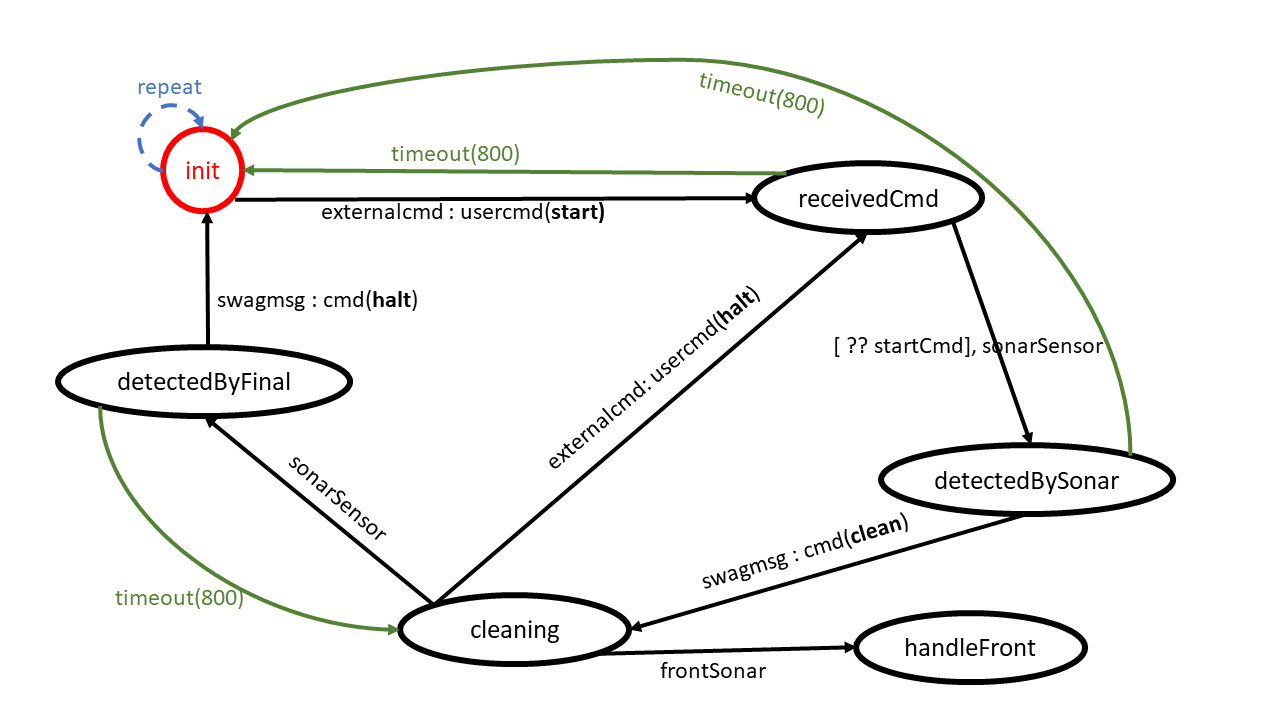
\includegraphics[scale=0.4]{img/stateDiagramStartStopEnd.png}
\caption{Diagramma parziale degli stati di \texttt{SoftwareAgent} - \code{R-Start}, \code{R-Stop} e \code{R-End}}\labelfig{fsmStartStopEnd}
\end{figure}

\subsection{Cleaning the room}
Durante la sua attività, il robot deve pulire l'intera superficie della stanza (\code{R-FloorClean}). L'approccio più semplice per affrontare la pulizia di una stanza rettangolare è quello di partire da un angolo e percorrere a ''zig-zag'' la stanza in tutta la sua profondità, coprendo progressivamente l'intera larghezza fino a terminare nell'angolo opposto a quello di partenza.

I movimenti del robot possono essere quindi riassunti in prima battuta dal diagramma della \xf{floorCleanDraft}

\begin{figure}[!htb]
\centering
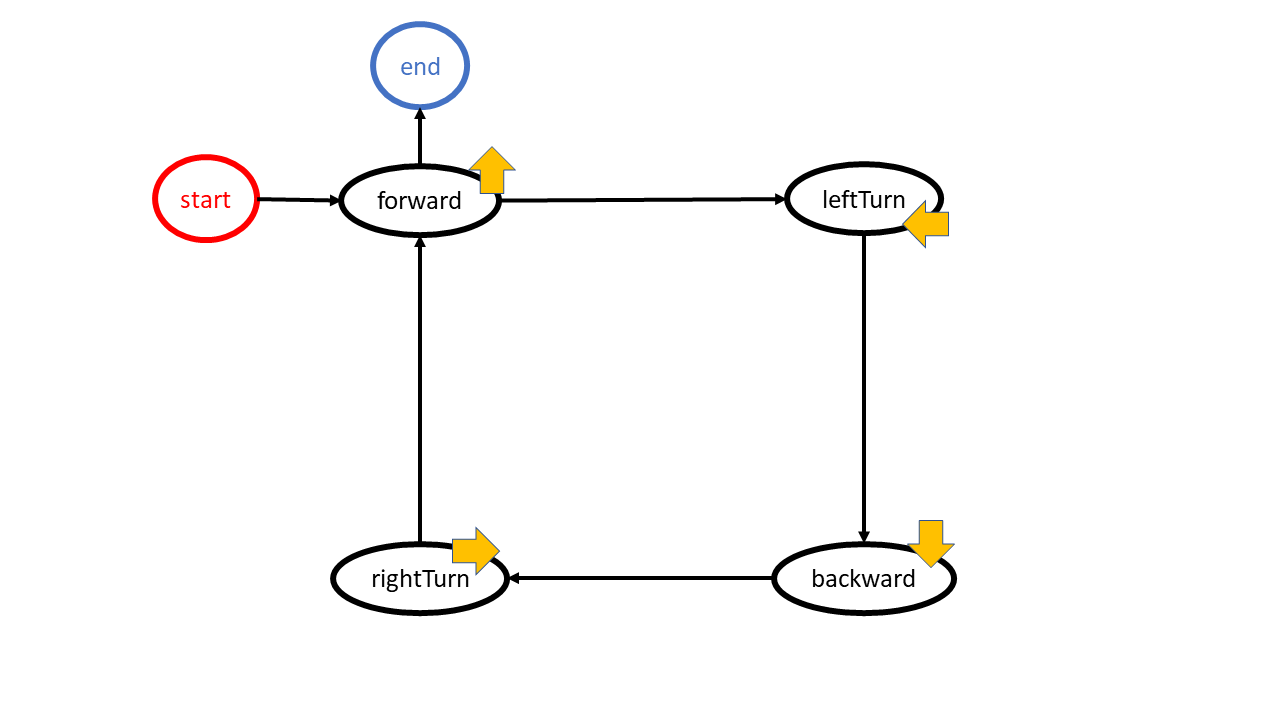
\includegraphics[scale=0.45]{img/stateDiagramCleaningDraft.png}
\caption{Schema del movimento del robot durante la pulizia}\labelfig{floorCleanDraft}
\end{figure}

Partendo da questo modello concettuale di base, introduciamo alcuni stati aggiuntivi che derivano dai vincoli specifici del problema.

In particolare, mentre il raggiungimento della parete frontale (rispetto alla posizione iniziale del robot, ovvero quella opposta a \code{sonar1}) è segnalato dalla presenza del secondo sonar, per la parete di fondo non vi è altro modo se non il sonar frontale del robot a rilevare la presenza di un generico ostacolo. Questa problematica verrà ripresa nella sezione successiva.

Un'ulteriore complicazione riguarda la presenza del primo sonar lungo tutta la parete di sinistra, il che ci suggerisce l'inserimento di uno stato aggiuntivo, \texttt{startCleaning}, analogo allo stato di \texttt{forward}, dove anche in questo caso viene usato eccezionalmente il sonar frontale per gestire la svolta al raggiungimento della parete
\footnote{Assumiamo, per semplicità, che non vi siano ostacoli lungo le pareti}.

\begin{qacode}[caption={SoftwareAgent, pt5}]
Plan startCleaning [
	println("start cleaning");
	emit inputCtrlEvent : inputEvent( agent,swag,cleaning ); // (1)
	forward controller -m cmd : cmd( w(0) )
]
transition stopAfter 3600000
	whenEvent frontSonar -> leftTurn,
	whenEvent externalcmd -> receivedCmd // R-Stop
	
Plan leftTurn [
	println("left turn");	
	forward controller -m cmd : cmd( h(0) );
	forward controller -m cmd : cmd( a(0) );
	delay 1000;
	forward controller -m cmd : cmd( w(0) );
	delay 800;
	forward controller -m cmd : cmd( h(0) );
	forward controller -m cmd : cmd( a(0) );
	delay 800
]
switchTo backCleaning

Plan backCleaning [
	println("cleaning back");
	forward controller -m cmd : cmd( w(0) )
]
transition stopAfter 3600000
	whenEvent frontSonar -> rightTurn,
	whenEvent externalcmd -> receivedCmd // R-Stop
	
Plan rightTurn [
	println("right turn");
	forward controller -m cmd : cmd( h(0) );
	forward controller -m cmd : cmd( d(0) );
	delay 1000;
	forward controller -m cmd : cmd( w(0) );
	delay 800;
	forward controller -m cmd : cmd( h(0) );
	forward controller -m cmd : cmd( d(0) );
	delay 800
]
switchTo forwardCleaning

Plan forwardCleaning [
	println("cleaning forward");
	forward controller -m cmd : cmd( w(0) )
]
transition stopAfter 3600000
	// la parete di fondo e' segnalata da sonar2
	whenEvent sonarSensor -> detectedByFinal, // R-End
	whenEvent externalcmd -> receivedCmd // R-Stop
\end{qacode}

Dallo stato \codescript{detectedByFinal}, riportato precedentemente, l'agent transita infine nello stato finale \codescript{end}.\\

\begin{qacode}[caption={SoftwareAgent, pt5}]
Plan end [
	println("end");
	emit inputCtrlEvent : inputEvent( agent,swag,idle ); // (2)
	forward controller -m cmd : cmd( h(0) )
]
switchTo init
\end{qacode}

Quando il robot viene pilotato da un utente umano, in caso di collisione è il controller a rilevare l'evento \codescript{frontSonar} e a fermare il robot. Ciò non deve accadere quando è invece il \texttt{SoftwareAgent} a controllarlo: per questo motivo l'agent si fa carico di inviare un \codescript{inputCtrlEvent} per segnalare al controller quando sta pilotando il robot, così che questi non interferisca (righe (1) e (2)).

Alla ricezione di questi eventi, il controller modifica il modello delle risorse in cui è mantenuto lo stato dell'agent.\\

\begin{lstlisting}[language=Prolog, keywordstyle=\color{black}, caption={resourceModel.pl}]
% Modello dell'agent
model( type(software, agent), name(swag), value(idle) ).
\end{lstlisting}

\begin{qacode}[caption={Gestione di \codescript{frontSonar} da parte del \texttt{Controller}}]
Plan handleFront resumeLastPlan [
	[ !? getModelItem( software,agent,swag,idle ) ]
		demo changeRobotModel(h(0))
]
\end{qacode}

Il diagramma degli stati risultante è quindi rappresentato nella \xf{floorClean}

\begin{figure}[!htb]
\centering
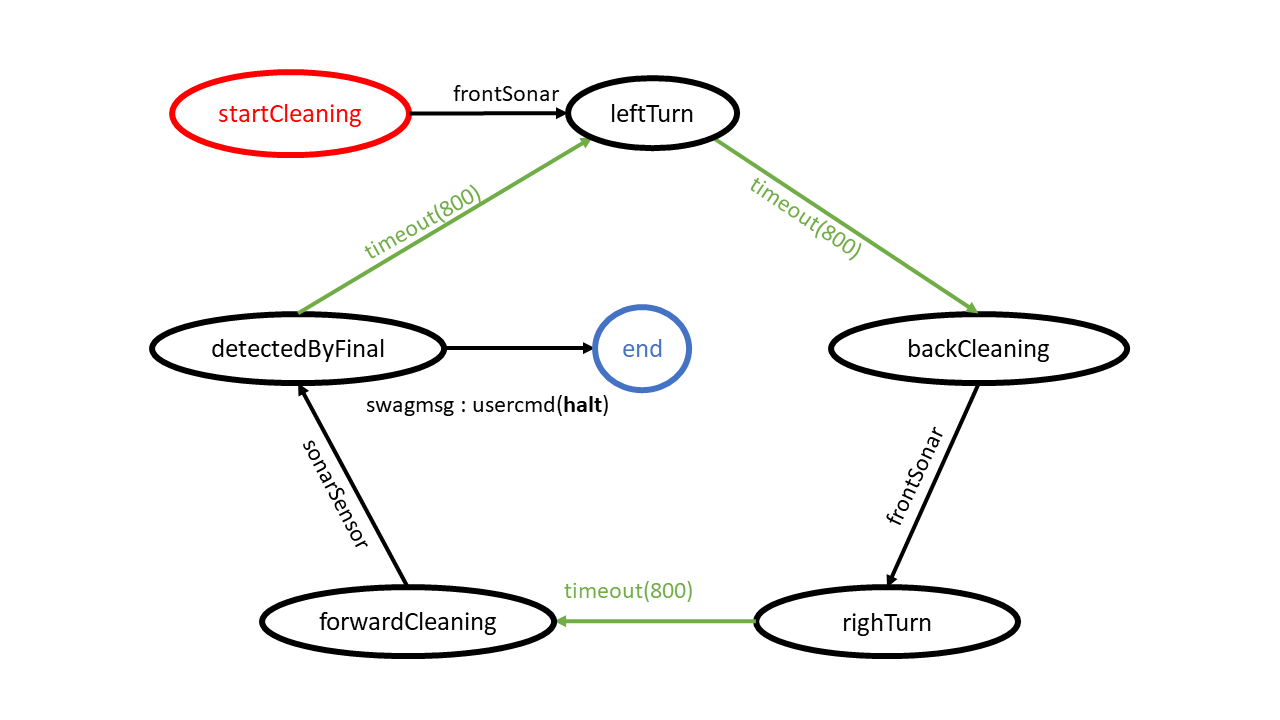
\includegraphics[scale=0.4]{img/stateDiagramCleaning.png}
\caption{Diagramma parziale degli stati di \texttt{SoftwareAgent} - \code{R-FloorClean}, \code{R-End}}\labelfig{floorClean}
\end{figure}

\subsection{Obstacle avoidance}
Gli eventi \codescript{frontSonar} permettono al  \texttt{SoftwareAgent} di individuare gli ostacoli sul cammino del robot. In presenza di uno di questi deve cercare di capire se sia fisso o mobile e tentare di evitarlo.

Inizialmente si assume che l'ostacolo sia mobile, si aspetta dunque un piccolo intervallo di tempo per poi riprovare ad avanzare. Se non si ricevono altri eventi dal sonar frontale, si presume di essere riusciti a superare l'ostacolo.\\

\begin{qacode}[caption={SoftwareAgent, pt6}]
Plan handleFront [
	println("handleFront");
	forward controller -m cmd : cmd( h(0) );
	println("possible mobile obstacle");
	delay 1000;
	forward controller -m cmd : cmd( w(0) );
	println("provo ad avanzare")
]
transition
	whenTime 800 -> avoidMobile
	whenMsg externalcmd -> receivedCmd,
	whenEvent frontSonar -> avoidFix // R-AvoidFix
 
 // R-AvoidMobile
 Plan avoidMobile [
	println("avoidMobile");
	println("ok, ostacolo superato")
]
switchTo cleaning
\end{qacode}

Viceversa, se si ricevono altri eventi \codescript{frontSonar}, l'ostacolo viene considerato fisso e occorre provare ad aggirarlo prima da una direzione e, in caso di fallimento, dall'altra, cercando periodicamente la presenza di passaggi.\\

\begin{qacode}[caption={SoftwareAgent, pt7}]
Plan avoidFix [
	println("avoidFix");
	forward controller -m cmd : cmd( h(0) );
	[ !? exploring(DIR) ] println(explorng(DIR))
	else addRule exploring(r);
	// aumento contatore di tentativi
	demo avoidFixTry;
	[ !? avoidFixGiveUp ] {
		[ !? exploring(l) ] selfMsg swagmsg : cmd(giveUpLeft) // R-Obstacle
		else selfMsg swagmsg : cmd(giveUpRight);
		demo switchExplorationDir;
		println("Raggiunti max tentativi")
	} else {
		delay 800;
		println("proviamo a girarci intorno");
		[ !? exploring(l) ] {
			forward controller -m cmd : cmd( a(0) );
			println("da sinistra")
		}
		else {
			forward controller -m cmd : cmd( d(0) );
			println("da destra")
		};
		delay 2000;
		forward controller -m cmd : cmd( w(0) );
		delay 1000; // passo laterale
		forward controller -m cmd : cmd( h(0) );
		delay 2000
	}
]
transition
	whenTime 800 -> checkDoor
	whenEvent frontSonar -> failure,
	whenMsg externalcmd -> receivedCmd,
	whenMsg swagmsg -> giveUp // esaminare il payload

Plan checkDoor [
	println("checkDoor");
	[ !? exploring(r) ] forward controller -m cmd : cmd( a(0) )
	else forward controller -m cmd : cmd( d(0) );
	delay 800;
	forward controller -m cmd : cmd( w(0) );
	delay 800;
	forward controller -m cmd : cmd( h(0) );
	delay 2000
]
transition
	whenTime 800 -> doorFound
	whenMsg externalcmd -> receivedCmd,
	whenEvent frontSonar -> avoidFix

Plan doorFound [
	println("doorFound");
	forward controller -m cmd : cmd( w(0) );
	delay 1000;
	forward controller -m cmd : cmd( h(0) );
	[ !? exploring(r) ] forward controller -m cmd : cmd( a(0) )
	else forward controller -m cmd : cmd( d(0) )
]
switchTo goToPrevLevel
\end{qacode}

Il fallimento è determinato dalla presenza di un nuovo ostacolo che impedisce di proseguire oltre in quella direzione o dopo un certo numero di tentativi non riusciti. Se si fallisce in entrambe le direzioni, la pulizia termina (\code{R-Obstacle}).\\

\begin{qacode}[caption={SoftwareAgent, pt8}]
Plan failure [
	println("failure");
	[ !? exploring(r) ] {
		println("failure da destra");
		selfMsg swagmsg : cmd(giveUpRight);
		delay 800;
		forward controller -m cmd : cmd( a(0) )
	}
	else {
		selfMsg swagmsg : cmd(giveUpLeft);
		println("failure da sinistra")
	};
	demo switchExplorationDir
]
transition stopAfter 3600000
	whenMsg swagmsg -> giveUp

// ho raggiunto max tentativi
Plan giveUp [
	println("giveUp");
	// elimino l'ultimo incremento, quello che ha fatto raggiungere la soglia
	demo decremFoundFix;
	onMsg swagmsg : cmd(giveUpRight) -> {
		delay 800;
		forward controller -m cmd : cmd( a(0) );
		delay 800;
		selfMsg swagmsg : cmd(resumeLastPos)
	};
	onMsg swagmsg : cmd(giveUpLeft) -> { // R-Obstacle
		removeRule foundFix(X);
		removeRule exploring(l)
	}
]
transition
	whenTime 800 -> end
	whenMsg swagmsg -> resumeLastPosition
	
Plan resumeLastPosition [
	println("resume last position");
	delay 2000;
	[ !? counter(foundFix,C) ] {
		demo decremFoundFix;
		forward controller -m cmd : cmd( w(0) );
		delay 800;
		forward controller -m cmd : cmd( h(0) );
		delay 2000
	}
	else {
		selfMsg swagmsg : cmd(initialP); // raggiunta posizione di partenza
		forward controller -m cmd : cmd( d(0) )
	}
]
transition
	whenTime 800 -> resumeLastPosition
	whenMsg externalcmd -> receivedCmd,
	whenMsg swagmsg -> avoidFix
\end{qacode}

Se invece viene trovato un passaggio, dopo averlo superato il robot deve ritornare alla stessa altezza a cui si trovava prima dell'ostacolo.\\

\begin{qacode}[caption={SoftwareAgent, pt9}]
Plan goToPrevLevel [
	println("goToPrevLevel");
	delay 2000;
	[ !? counter(foundFix,C) ] {
		demo decremFoundFix;
		forward controller -m cmd : cmd( w(0) );
		delay 800;
		forward controller -m cmd : cmd( h(0) )
	}
	else {
		selfMsg swagmsg : cmd(initialP); // raggiunta posizione di partenza
		[ !? exploring(r) ] forward controller -m cmd : cmd( d(0) )
		else forward controller -m cmd : cmd( a(0) );
		delay 800;
		println("riprendo la direzione di marcia")
	}
]
transition
	whenTime 300 -> goToPrevLevel
	whenMsg externalcmd -> receivedCmd,
	whenMsg swagmsg -> cleaning
\end{qacode}

Gli stati che implementano le politiche di \emph{obstacle avoidance} possono essere riassunti con la \xf{obstacleAvoidance}.

\begin{figure}[!htb]
\centering
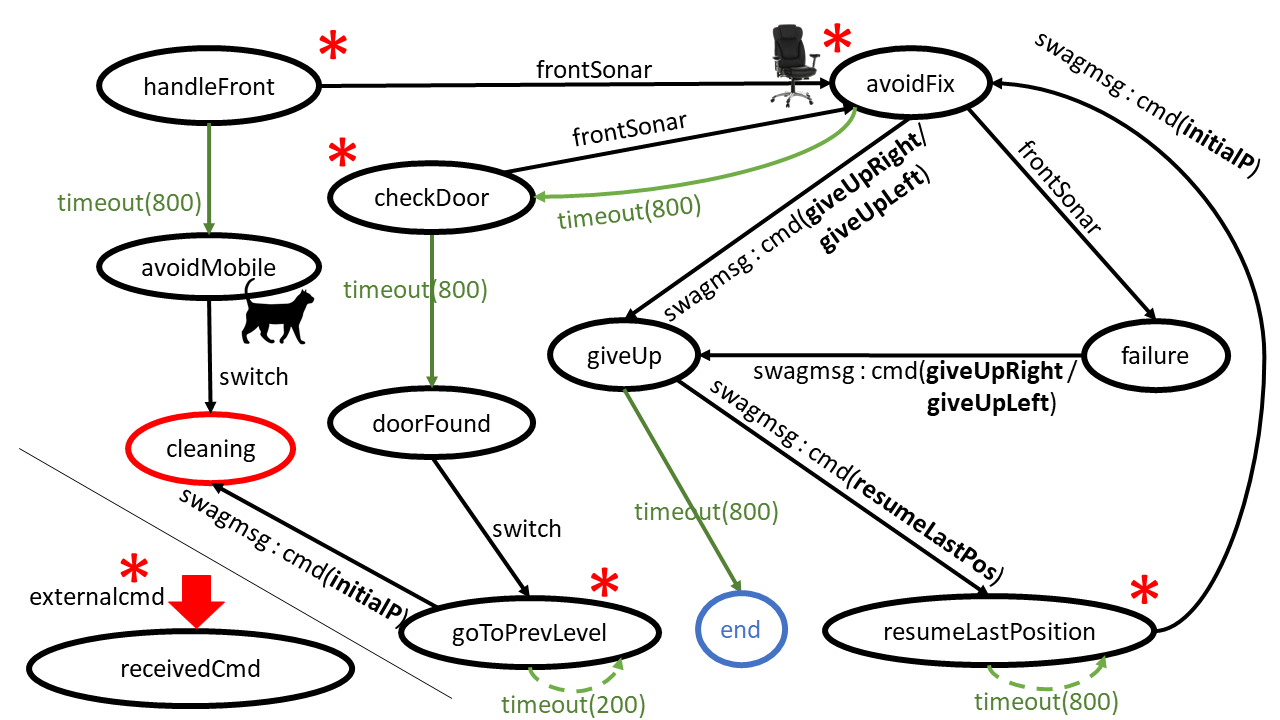
\includegraphics[scale=0.4]{img/stateDiagramObstacle.png}
\caption{Diagramma parziale degli stati di \texttt{SoftwareAgent} - \code{R-AvoidFix}, \code{R-AvoidMobile}, \code{R-Obstacle}}\labelfig{obstacleAvoidance}
\end{figure}

Per gestire il passaggio fra i suoi stati interni, l'agent utilizza dei messaggi ''privati'' \codescript{swagmsg : cmd(CMD)}, mentre le due fasi di esplorazione, a destra e a sinistra dell'ostacolo, vengono realizzate dagli stessi stati discriminando i due casi tramite la regola \codescript{exploring(DIR)}.\\

\begin{lstlisting}[language=Prolog, keywordstyle=\color{black}, caption={SoftwareAgent, Rules - pt2}]
switchExplorationDir :-
	exploring(r),
	retract(exploring(r)),
	assert(exploring(l)).
\end{lstlisting}

Per realizzare il comportamento a tentativi del robot vengono impiegate le seguenti regole Prolog che implementano un contatore.\\

\begin{lstlisting}[language=Prolog, keywordstyle=\color{black}, caption={SoftwareAgent, Rules - pt3}]
increment(C) :-
	counter(C,N), !,
	N2 is N+1,
	retract(counter(C,N)),
	assert(counter(C,N2)).
	
increment(C) :-
	assert(counter(C,1)).
	
increment(C,1) :- !,
	increment(C).
	
increment(C,N) :-
	increment(C),
	eval(minus,N,1,N2),
	increment(C,N2).

decrement(C) :-
	counter(C, 1), !,
	retract(counter(C, 1)).

decrement(C) :-
	counter(C,N), !,
	eval(minus, N, 1, N2),
	retract(counter(C,N)),
	assert(counter(C,N2)).

avoidFixTry :-
	increment(foundFix).

avoidFixGiveUp :-
	counter(foundFix, 3).

decremFoundFix :-
	decrement(foundFix).
\end{lstlisting}

\subsection{Complete Agent}
Per integrare l'\emph{obstacle avoidance} con la pulizia della stanza sono necessari alcuni accorgimenti.\\

Poiché abbiamo assunto che non vi siano ostacoli lungo le pareti, gli unici stati sensibili agli eventi del sonar frontale sono \codescript{forwardCleaning} e \codescript{backCleaning}, ai quali va quindi aggiunta la transizione che originariamente si trovava nello stato fittizio \emph{cleaning}.

Inoltre, dopo aver aggirato un ostacolo, l'agent deve tornare nello stato in cui si trovava in precedenza: a tal fine abbiamo introdotto lo stato \codescript{selectDirection}, che tramite opportune regole discrimina lo stato futuro in cui deve portarsi. Tali regole devono essere asserite nei rispettivi stati di provenienza.\\

\begin{qacode}[caption={SoftwareAgent, pt10}]
Plan selectDirection [
	println("selectDirection");
	removeRule exploring(X);
	[ !? direction(f) ] println("f");
	[ !? direction(b) ] { println("b"); selfMsg swagmsg : cmd(b) }
]
transition
	whenTime 800 -> forwardCleaning
	whenMsg swagmsg -> backCleaning
	
Plan forwardCleaning [
	println("cleaning forward");
	[ !? direction(D) ]
		println(direction(D)) // debug
	else
		addRule direction(f);
	forward controller -m cmd : cmd( w(0) )
]
transition stopAfter 3600000
	whenEvent sonarSensor -> detectedByFinal, // R-End
	whenEvent frontSonar -> handleFront,
	whenEvent externalcmd -> receivedCmd // R-Stop

Plan backCleaning [
	println("cleaning back");
	[ !? direction(D) ]
		println(direction(D)) // debug
	else
		addRule direction(b);
	forward controller -m cmd : cmd( w(0) )
]
transition stopAfter 3600000
	whenEvent frontSonar -> frontSonarDetected,
	whenEvent externalcmd -> receivedCmd // R-Stop
\end{qacode}

Per distinguere la parete di fondo da un ostacolo, entrambi segnalati da un evento \codescript{frontSonar}, utilizziamo un contatore per misurare la profondità della stanza durante il primo tratto, corrispondente a \codescript{startCleaning}, e uno durante ogni pulizia ''backward''. In questo modo, alla ricezione dell'evento, è possibile capire se si debba tornare indietro (\emph{turnRight}) o evitare l'ostacolo.\\

\begin{qacode}[caption={SoftwareAgent, pt11}]
Plan startCleaning [
	[...]
]
switchTo countRoomLen

Plan countRoomLen [
	demo increment(roomLen) // counter(roomLen, C++)
]
transition
	whenTime 300 -> countRoomLen
	whenEvent frontSonar -> leftTurn,
	whenEvent externalcmd -> receivedCmd // R-Stop
	
Plan backCleaning [
	[...]
]
switchTo countSteps

Plan countSteps [
	demo increment(steps) // counter(steps, C++)
]
transition
	whenTime 300 -> countSteps
	whenEvent frontSonar -> frontSonarDetected,
	whenEvent externalcmd -> receivedCmd // R-Stop
	
Plan frontSonarDetected [
	println("frontSonarDetected");
	[ !? counter(roomLen,C)] println(roomLen(C));
	[ !? counter(steps,N)] println(steps(N));
	
	[ !? isInWallProximity ] {
		println("parete");
		[ !? direction(b) ] selfMsg swagmsg : cmd(r)
	}
	else
		println("ostacolo")
]
transition
	whenTime 800 -> handleFront // obstacle avoidance
	whenMsg swagmsg -> rightTurn // wall
\end{qacode}

Se i passi contati sono maggiori o minori entro una certa soglia (per tolleranza ad eventuali errori nel conteggio) della dimensione della stanza, allora il robot si trova davanti alla parete di fondo.\\

\begin{lstlisting}[language=Prolog, keywordstyle=\color{black}, caption={SoftwareAgent, Rules - pt4}]
isInWallProximity :-
	counter(steps,N),
	counter(roomLen,M),
	eval(minus,M,N,R),
	eval(lt,R,4).
\end{lstlisting}

Per quanto riguarda il raggiungimento della parete frontale, segnalata dalla presenza di \code{sonar2}, occorre tenere in considerazione il fatto che il robot potrebbe comunque urtare la parete, generando un evento \codescript{frontSonar}. Se tale evento viene ricevuto quando l'agent si trova già in \codescript{backCleaning}, questi potrebbe scambiarlo erroneamente per un ostacolo. Pertanto, abbiamo inserito uno stato ''di comodo'' per catturare l'eventuale \codescript{frontSonar} e ''consumarlo'' prima di transitare in uno stato sensibile agli eventi del sonar frontale
\footnote{
\url{https://en.wikipedia.org/wiki/Waiting_for_Godot}
}.\\

\begin{qacode}[caption={SoftwareAgent, pt12}]
Plan leftTurn [
	[...]
]
transition
	whenTime 800 -> waitForGodot

// "consumo" eventuali eventi frontSonar residui...
Plan waitForGodot [
	println("waiting for Godot...")
]
transition
	whenTime 2000 -> backCleaning // tutto ok, procedi
	whenEvent frontSonar -> backCleaning // evento "consumato"
\end{qacode}
%===========================================================================

%===========================================================================
\section{Implementation}
\labelsec{Implementation}

\subsection{Hue Lamp Interaction}
L'interazione con la Hue Lamp Philips avviene mediante un'interfaccia di API RESTful\footnote{\url{https://it.wikipedia.org/wiki/Representational_State_Transfer}} fornita dall'apposito bridge.

Prima di interagire con la lampada, è quindi necessario individuare il bridge nella rete ed ottenere uno username. Sempre grazie alla documentazione apprendiamo che entrambe le operazioni possono essere facilmente svolte con messaggi HTTP: la prima attraverso una GET ad un preciso url (\url{https://discovery.meethue.com/}), mentre la seconda grazie alle API del bridge individuato con la prima.\\

Attualmente il nostro sistema simula la lampada Wi-Fi con un oggetto mock scritto in Java; ci viene quindi facile sostituirlo mediante un'altra classe Java che funga da adapter per le API del sistema Hue Lamp Philips.\\

\lstinputlisting[language=Java, firstline=20, lastline=70, firstnumber=20]{../it.unibo.finaltask2018/src/it/unibo/finaltask2018/adapter/hueLampAdapter.java}

Tale classe espone i due metodi statici \codescript{setUp()} e \codescript{setLamp(String state)}: il primo esegue le operazioni per stabilire una connessione col bridge ed ottenere le credenziali, mentre il secondo è un metodo adapter per chiamare le API che permettono di cambiare lo stato della lampadina (on/off/blink).\\

Dal momento che sia l'interazione con la lampada, sia le operazioni preliminari per individuare l'indirizzo IP del bridge nella rete e per l'ottenimento dello username sono gestite attraverso comunicazione RESTful, abbiamo implementato una classe Java di utilità\footnote{RESTfulClient.java} che, sfruttando un'apposita libreria, semplifichi tali operazioni.
Anche per quanto riguarda la scrittura/lettura dei dati in JSON ci siamo appoggiati ad una libreria.

\subsection{Virtual Robot with Node.js}
\labelssec{robotNodeImpl}
L'implementazione del robot virtuale si basa sul progetto \texttt{configurable-threejs-app}\footnote{\url{https://github.com/PierfrancescoSoffritti/configurable-threejs-app}} di Pierfrancesco Soffritti, il quale fa uso di un server Node.js che può essere raggiunto sia tramite browser, sia tramite una semplice connessione TCP.

Come prima cosa quindi, il nostro robot modellato tramite il linguaggio \qa (\xss{virtualRobotPA}) deve occuparsi di avviare il server e stabilire con questi una connessione.\\

\lstinputlisting[style=style_qa, firstline=21, lastline=35, firstnumber=21]{../it.unibo.finaltask2018/src/virtualRobotNode.qa}

La classe Java fa uso di un file \texttt{.bat} per eseguire il server in un nuovo terminale, appositamente aperto, evitando così che questa operazione debba essere fatta manualmente dall'utente, ma allo stesso tempo lasciando all'utilizzatore il controllo per poterlo terminare.\\

\lstinputlisting[language=Java, firstline=6, lastline=30, firstnumber=6]{../it.unibo.finaltask2018/src/it/unibo/finaltask2018/robot/NodeRobot.java}

L'implementazione dei metodi che corrispondono alle varie mosse fa uso della classe di utilità \codescript{it.unibo.utils.clientTcp}, la quale costruisce i messaggi nel giusto formato accettato dal server e li invia sulla connessione TCP.

Inoltre, da questa un thread dedicato legge continuamente i dati in arrivo, corrispondenti alle informazioni emesse dai sonar fissi e mobili, per poi emettere i relativi eventi \codescript{sonarSensor} e \codescript{frontSonar}.

\subsection{Real Robot with Arduino+RaspberryPi}
Il robot fisico che si trova sul RaspberryPi\footnote{progetto: \texttt{it.unibo.raspRobot}} interagisce con il resto del sistema tramite l'invio e la ricezione di eventi (propagati dall'infrastruttura \qa via rete) e con Arduino -- dove sono collegati sensori e attuatori -- tramite una connessione seriale.

L'architettura del sistema può essere quindi riassunta dalla \todo{riferimento}.

In realtà, il robot non comunica direttamente con Arduino, in quanto abbiamo scelto di introdurre un ulteriore strato software che esponga una visione di alto livello dei dispositivi fisici collegati alla board di Arduino: questi sono presentati come servizi accessibili via rete (TCP) e gestiti da un opportuno server Python, il quale è l'unico a leggere e scrivere dati sulla seriale (lato Raspberry).

Questa soluzione scarica dal robot fisico la responsabilità di conoscere i dettagli della comunicazione con Arduino, a favore di un'interazione tra entità di alto livello (micro-servizi).\\

\lstinputlisting[style=style_qa]{../it.unibo.raspRobot/src/realrobot.qa}

L'attore che rappresenta il robot utilizza un'apposita classe Java che si comporta come un client nei confronti del server Python, inviando i comandi di movimento e ricevendo da questi i dati relativi al sonar frontale.

L'architettura risultante è rappresentata nella \todo{riferimento}.

% .qa, differenze (minime) rispetto al modello della PA
% spiegare mapping comandi?

\subsubsection{Temperature from a real sensor}
Una possibile implementazione del servizio che fornisce la temperatura può essere basata su un sensore fisico collegato ad uno degli ingressi analogici di Arduino.

Anche in questo caso si tratta sempre del gestore della connessione seriale scritto in Python a fornire i dati all'esterno, mettendo a disposizione degli utilizzatori un server in grado di rispondere, su richiesta, con l'informazione della temperatura corrente.

% listing python?

% subsubsection arduino?
%===========================================================================

%===========================================================================
\section{Testing}
\labelsec{Testing}

Per quanto riguarda il testing, l'approccio adottato è principalmente a \emph{black-box}, ovvero senza assumere di avere nozione di quale sia l'effettivo comportamento interno del componente sotto esame, concentrando invece l'attenzione sull'aspetto dell'interazione. Questo consente di strutturare i test in maniera indipendente dalle specifiche implementazioni e, in alcuni casi, di riutilizzare gli stessi test durante le varie fasi dello sviluppo.\\

I test seguono un ordine incrementale del tipo bottom-up, partendo cioè dalle singole unità (\emph{unit testing}), per passare poi all'integrazione di queste (\emph{integration testing}) e, infine, ai vari sottosistemi e ai servizi da essi offerti (\emph{functional testing}).

Queste prime tre tipologie di test possono essere eseguite in maniera automatica facendo uso del framework \texttt{JUnit}, mentre lo \emph{user acceptance testing} viene condotto manualmente man mano che un nuovo componente viene aggiunto al sistema.\\

Una struttura ricorrente nei test è la verifica, in seguito al verificarsi di alcune circostanze, di cosa è presente o no nella base di conoscenza di certi attori. Nonostante per fare ciò tali QActor vengano trattati come dei semplici oggetti Java, occorre tenere presente che in realtà ognuno di essi rappresenta un flusso di controllo autonomo, pertanto è caratterizzato da tempi di avvio propri, da tempi di transizione da uno stato all'altro, eccetera.

L'utilizzo estensivo di opportune \codescript{sleep} non preclude quindi la possibilità di eventuali fallimenti dovuti all'impredicibilità dell'ordine di scheduling.

\subsection{Requirement analysis}
\labelsssec{reqAnalTesting}

\subsubsection{Led unit test}
Il testing del led prevede di verificare semplicemente il comportamento dei metodi esposti nell'interfaccia \codescript{ILed} (\xss{actuatorsRA}). Anche se nello specifico è stato usato un oggetto mock provvisto di GUI per simulare il led fisico, il test rimane valido per qualsiasi implementazione dell'interfaccia.\\

\lstinputlisting[language=Java, firstline=12, lastline=31, firstnumber=12]{../it.unibo.finalTask2018/test/it/unibo/test/ra/LedTest.java}

\subsubsection{HueLampAgent unit test}
L'\codescript{HueLampAgent} riceve eventi \codescript{lightCmd} e li traduce in comandi per la Hue Lamp remota. Poiché in questo caso l'oggetto del testing è il comportamento dell'agent e non la comunicazione tra questi e la Hue Lamp, possiamo limitarci a controllare che alla ricezione di un evento corrisponda un effettivo cambiamento di stato nell'oggetto Java che simula la lampada.\\

\lstinputlisting[language=Java, firstline=15, lastline=41, firstnumber=15]{../it.unibo.finalTask2018/test/it/unibo/test/ra/HueLampAgentTest.java}

\subsubsection{TemperatureAgent unit test}
Lo scopo di \codescript{TemperatureAgent} è quello di emettere periodicamente eventi \codescript{temperature}. Dobbiamo quindi verificare che, dopo un tempo ragionevole, questi siano stati effettivamente generati e che i dati sulla temperatura in essi contenuti corrispondano a quanto rilevato dal sensore.\\

\lstinputlisting[language=Java, firstline=15, lastline=28, firstnumber=15]{../it.unibo.finalTask2018/test/it/unibo/test/ra/TemperatureAgentTest.java}

Per registrare gli eventi emessi nel sistema è stato usato un \emph{event logger} event-driven:\\

\lstinputlisting[style=style_qa, firstline=12, lastline=15, firstnumber=12]{../it.unibo.finalTask2018/src/requirementsAnalysis.qa}

\lstinputlisting[style=style_qa, firstline=123, lastline=129, firstnumber=123]{../it.unibo.finalTask2018/src/requirementsAnalysis.qa}

Il comportamento da attuare alla ricezione di un evento è precisato in un file Prolog esterno, così che possa essere condiviso da più event logger.\\

\lstinputlisting[language=Prolog, keywordstyle=\color{black}, firstline=6]{../it.unibo.finalTask2018/logger.pl}

\subsubsection{ClockAgent unit test}
Un ragionamento analogo al precedente vale anche per il testing di \codescript{ClockAgent}:\\

\lstinputlisting[language=Java, firstline=15, lastline=29, firstnumber=15]{../it.unibo.finalTask2018/test/it/unibo/test/ra/ClockAgentTest.java}

\subsubsection{HumanOperator and Application logic integration test}
Poiché lo \codescript{HumanOperator} è un attore che emette comandi per il robot nella forma di messaggi per il componente che incapsula la logica applicativa, il testing del primo è legato a quello della seconda.

Nello specifico, occorre verificare che quest'ultima emetta i rispettivi eventi \codescript{robotCmd} per il robot e \codescript{lightCmd} per il led/la Hue Lamp. A tal scopo ricorriamo ancora una volta all'event logger.\\

\lstinputlisting[language=Java, firstline=14, lastline=44, firstnumber=14]{../it.unibo.finalTask2018/test/it/unibo/test/ra/HumanOpApplTest.java}

Si noti come i primi due test facciano riferimento ai messaggi inviati a fine di testing direttamente nel modello dell'analisi dei requisiti (\xss{humanOpRA}).

\subsubsection{Robot unit test}
Il robot, sia fisico sia virtuale, è stato modellato come un attore in grado di interpretare messaggi \codescript{moveRobot} e tradurli in opportune azioni di movimento. Oltre a questo, il robot è sensibile agli eventi \codescript{robotCmd} generati dalla logica applicativa e mappati in messaggi da un \codescript{EventHandler}.

Infine, il robot può emettere informazioni relative al sonar frontale e al proprio passaggio in corrispondenza di uno dei due sonar presenti nella stanza.\\

Il testing si concentrerà quindi su questi tre aspetti, verificando lo stato del robot in seguito all'invio di comandi sotto forma di messaggi ed eventi, e consultando la base di conoscenza dell'event logger per controllare l'effettiva emissione degli eventi \codescript{frontSonar} e \codescript{sonarSensor}.\\

\lstinputlisting[language=Java, firstline=17, lastline=46, firstnumber=17]{../it.unibo.finalTask2018/test/it/unibo/test/ra/DdrTest.java}

\subsubsection{Robot \& Application system integration test}
Dopo aver testato che l'applicazione sia in grado di tradurre messaggi \codescript{cmd} in opportuni eventi \codescript{robotCmd} e \codescript{lightCmd}, e che il robot interpreti correttamente tali comandi, rimane da verificare che i due componenti continuino a funzionare una volta entrati a far parte di uno stesso sistema (\xss{formalRA}).\\

Per automatizzare il test occorre eseguire in processi distinti l'applicazione principale, il robot e, infine,
%\codescript{raintegrator.qa}, che funge da
il ``system integrator'' tra gli altri due.

In particolare, l'obiettivo è controllare che all'invio di un \codescript{cmd} diretto al componente che incapsula la logica applicativa, il robot mock agisca di conseguenza grazie alla propagazione degli eventi garantita dall'infrastruttura {\qa}.\\

\lstinputlisting[language=Java, firstline=20, lastline=67, firstnumber=20]{../it.unibo.finalTask2018/test/it/unibo/test/ra/DdrApplIntegrationTest.java}

\subsection{Problem analysis}

\subsubsection{Controller unit test}
Gran parte della logica del \texttt{Controller} è espressa sotto forma di regole Prolog inserite all'interno della base di conoscenza del relativo attore. Per testare queste regole dobbiamo quindi, come fatto in precedenza, sfruttare i metodi dell'oggetto Java corrispondente.\\

\lstinputlisting[language=Java, firstline=15, lastline=98, firstnumber=15]{../it.unibo.finalTask2018/test/it/unibo/test/pa/ControllerTest.java}

Un'altra serie di test riguardano l'aspetto dell'interazione. Nell'effettivo, il \texttt{Controller} interagisce con l'esterno tramite gli eventi \codescript{ctrlEvent} (alcuni dei quali sono convertiti in \codescript{lightCmd} da un apposito EventHandler), \codescript{inputCtrlEvent} e i messaggi \codescript{cmd}.\\

\lstinputlisting[language=Java, firstline=100, lastline=134, firstnumber=100]{../it.unibo.finalTask2018/test/it/unibo/test/pa/ControllerTest.java}

\subsubsection{Software Agent unit test}
Per il testing di \texttt{SoftwareAgent} occorre verificare che, in seguito all'emissione degli eventi generati dai sonar (quello frontale e i due fissi), vengano recapitati al controller opportuni messaggi \codescript{cmd}. L'effetto di questi si ripercuote poi sullo stato del modello del robot e sugli eventi \codescript{ctrlEvent} emessi per pilotarlo.\\

\lstinputlisting[language=Java, firstline=14, lastline=47, firstnumber=14]{../it.unibo.finalTask2018/test/it/unibo/test/pa/SwAgentTest.java}

\subsubsection{HumanOperator unit test}
Un ragionamento simile può essere fatto per \texttt{HumanOperator}: questa volta è all'emissione di eventi \codescript{usercmd} -- gli stessi originati dalla web GUI -- che deve seguire l'invio dei relativi messaggi \codescript{cmd}.\\

\lstinputlisting[language=Java, firstline=14, lastline=34, firstnumber=14]{../it.unibo.finalTask2018/test/it/unibo/test/pa/HumanOpTest.java}

\subsubsection{Architecture integration test}
Dopo aver testato separatamente i vari componenti definiti nell'analisi del problema, passiamo a testare il sistema nel suo complesso. In particolare, siamo interessati a verificare che l'introduzione del resource model e del relativo controller abbia rispettato i quattro punti descritti nella \xs{ProblemAnalysis}.

In altre parole, simulando il cambiamento di stato di un sensore ci aspettiamo che questo venga correttamente notificato al controller, così che questi possa aggiornarne il modello. Poi, in accordo con la logica applicativa, deve seguire una modifica del modello degli attuatori, la loro notifica da parte del controller e un effettivo riscontro sugli attuatori ``reali''.\\

\lstinputlisting[language=Java, firstline=20, lastline=55, firstnumber=20]{../it.unibo.finalTask2018/test/it/unibo/test/pa/ArchIntegrationTest.java}

In questo caso si è simulata la pressione di un pulsante sulla console, per poi controllare sia lo stato della lampada, sia quello del robot, in entrambi i casi facendo uso di oggetti mock. Da notare come quest'ultimo, poiché si trova in un contesto diverso, offra, a fine di testing, un semplice server TCP per permettere di verificare dall'esterno il proprio stato.

\subsubsection{Time, temperature and blinking functional test}
Il passo successivo è testare la correttezza dei requisiti ad ora soddisfatti: \code{R-TempOk}, \code{R-TempKo}, \code{R-TimeOk}, \code{R-TimeKo}, \code{R-BlinkLed} e \code{R-BlinkHue}.

Per farlo inviamo una serie di comandi di movimento al robot e, sotto opportune condizioni, verifichiamo che:
\begin{itemize}
\item Il robot si muova quando la temperatura è al di sotto della soglia (e l'orario entro l'intervallo), viceversa non si deve muovere (\code{R-TempOk}).
\item Il robot si muova quando l'orario è all'interno dell'intervallo (e la temperatura al di sotto della soglia), viceversa non si deve muovere (\code{R-TimeOk}).
\item Non appena la temperatura sale al di sopra della soglia, il robot deve fermarsi (\code{R-TempKo}).
\item Non appena l'orario esce dall'intervallo consentito, il robot deve fermarsi (\code{R-TimeKo}).
\item La lampada deve lampeggiare quando il robot è in movimento, altrimenti deve essere spenta (\code{R-BlinkHue}).
\end{itemize}

\lstinputlisting[language=Java, firstline=22, lastline=102, firstnumber=22]{../it.unibo.finalTask2018/test/it/unibo/test/pa/TimeTempFunctionalTest.java}

%===========================================================================

%===========================================================================
\section{Maintenance}
\labelsec{Maintenance}
%===========================================================================

%===========================================================================
\section{Deployment}
\labelsec{Deployment}
%===========================================================================
 
%===========================================================================
\section{Author}
\labelsec{Author}
%===========================================================================

\vskip.5cm
%%% \begin{figure}
\begin{tabular}{ | c |  }
\hline
  % after \\: \hline or \cline{col1-col2} \cline{col3-col4} ...
  Photo of the author 
  \\
\hline
   %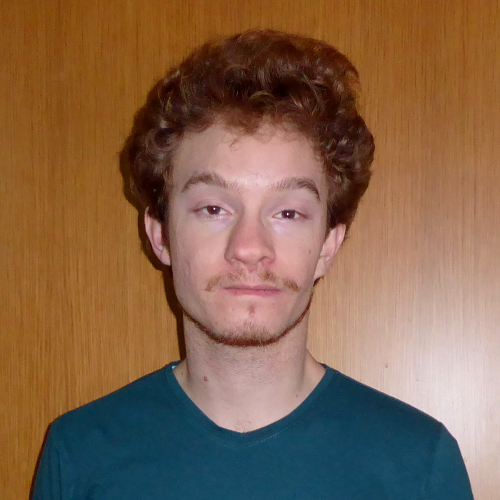
\includegraphics[scale = 0.7]{img/foto_autore.jpg}
   %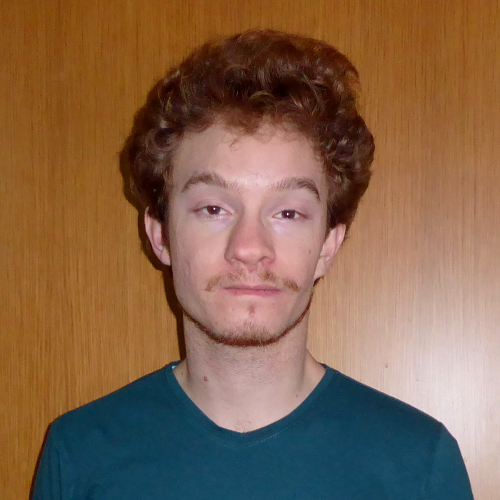
\includegraphics{img/foto_autore.jpg}
  \\
\hline
\end{tabular}
 
\end{document}
